\documentclass[graybox]{svmult}

% choose options for [] as required from the list
% in the Reference Guide

\usepackage{mathptmx}       % selects Times Roman as basic font
\usepackage{helvet}         % selects Helvetica as sans-serif font
\usepackage{courier}        % selects Courier as typewriter font
\usepackage{type1cm}        % activate if the above 3 fonts are
                             % not available on your system
%
\usepackage{makeidx}         % allows index generation
\usepackage{graphicx}        % standard LaTeX graphics tool
                             % when including figure files
\usepackage{multicol}        % used for the two-column index
\usepackage[bottom]{footmisc}% places footnotes at page bottom
\usepackage{latexsym,amsmath,amssymb,bm,booktabs,epsfig,multirow,bigstrut,graphicx,url,xspace,natbib}
%\usepackage{nath}

% see the list of further useful packages
% in the Reference Guide

\makeindex             % used for the subject index
                       % please use the style svind.ist with
                       % your makeindex program
                       
%\input FJHDef.tex
%\renewcommand{\bvec}[1]{\textbf{\itshape #1}}
%\renewcommand{\bvec}[1]{\boldsymbol{#1}}
\newcommand{\cube}{[0,1)^d}
\newcommand{\tcube}{\widetilde{[0,1)}^d}
\newcommand{\hv}{\hat{v}}
\newcommand{\fudge}{\mathfrak{C}}
\DeclareMathOperator{\MSE}{MSE}
\DeclareMathOperator{\RMSE}{RMSE}
\DeclareMathOperator{\rnd}{rnd}
\DeclareMathOperator{\abso}{abs}
\DeclareMathOperator{\rel}{rel}
\DeclareMathOperator{\nor}{nor}
\DeclareMathOperator{\err}{err}
%\DeclareMathOperator{\prob}{prob}
\DeclareMathOperator{\third}{third}
\DeclareMathOperator{\qse}{qse}
\DeclareMathOperator{\card}{card}
\DeclareMathOperator{\cost}{cost}
%\DeclareMathOperator{\fourth}{fourth}
%\newtheorem{theorem}{Theorem}
\spdefaulttheorem{algo}{Algorithm}{\upshape \bfseries}{\upshape}
%\newtheorem{algo}[theorem]{Algorithm}
%\newtheorem{rem}{Remark}
\DeclareMathOperator{\sMC}{sMC}
\newcommand{\aMC}{{\rm TwoStage}}


\newcommand\reals{\mathbb{R}}
\newcommand\real{\mathbb{R}}
\newcommand\natu{\mathbb{N}}
\newcommand\e{\mathbb{E}}
\newcommand{\bsx}{\boldsymbol{x}}
\newcommand{\vx}{\boldsymbol{x}}
\newcommand{\bsX}{\boldsymbol{X}}
\newcommand{\vX}{\boldsymbol{X}}
\newcommand{\rd}{\,\mathrm{d}}
\newcommand{\dnorm}{\mathcal{N}}
\newcommand{\Prob}{\Pr}

\newcommand{\abs}[1]{\left|#1\right|}
\DeclareMathOperator{\var}{Var}
\newcommand{\hmu}{\hat{\mu}}
\newcommand{\kurt}{\mathrm{kurt}}
\newcommand{\sign}{\mathrm{sign}}
\newcommand{\naturals}{\mathbb{N}}
\newcommand{\dif}{\rd}

\newcommand{\halpha}{\hat{\alpha}}
\newcommand{\hdelta}{\hat{\delta}}
\newcommand{\hvareps}{\hat{\varepsilon}}
\newcommand{\hsigma}{\hat{\sigma}}
\newcommand{\talpha}{\tilde{\alpha}}
\newcommand{\tdelta}{\tilde{\delta}}
\newcommand{\tkappa}{\tilde{\kappa}}
\newcommand{\tmu}{\tilde{\mu}}
\newcommand{\cb}{\mathcal{B}}
\newcommand{\fc}{\mathfrak{C}}
\newcommand{\cc}{\mathcal{C}}
\newcommand{\cf}{\mathcal{F}}
\newcommand{\cl}{\mathcal{L}}
\def\abs#1{\ensuremath{\left \lvert #1 \right \rvert}}
\newcommand{\norm}[2][{}]{\ensuremath{\left \lVert #2 \right \rVert}_{#1}}


\begin{document}


\date{\today}
\title*{Approximate Fixed Width Confidence Intervals Via Monte Carlo Sampling
\thanks{The first and second authors were partially supported by the National
Science Foundation under DMS-0923111 and DMS-1115392}}
\titlerunning{Fixed Width Confidence Intervals}
\author{Fred J. Hickernell\inst{1} \and
Lan Jiang\inst{1} \and Yuewei Liu\inst{2} \and Art Owen \inst{3}}
\institute{Department of Applied Mathematics,
Illinois Institute of Technology, Chicago, IL, USA,
\texttt{hickernell@iit.edu,ljiang14@hawk.iit.edu}
\and
School of Mathematics and Statistics, Lanzhou University, Lanzhou City, Gansu, China 730000, \texttt{???}
\and 
Art's address here \texttt{with email here}
}
%
% Use the package "url.sty" to avoid
% problems with special characters
% used in your e-mail or web address
%
\maketitle

\abstract{{\bf When we are done, we will write this.}}


\section{Introduction}

Monte Carlo algorithms provide a flexible way to approximate $\mu = \e(Y)$ when one can generate samples of the random variable $Y$. For example, $Y$ might be the discounted payoff of some financial derivative, which depends on the future performance of assets that are described by a stochastic model.  Then $\mu$ is the fair option price.  The goal is to obtain a \emph{confidence interval} 
\begin{equation} \label{confint}
\Prob[\abs{\mu - \hmu_n} \le \varepsilon] \ge 1-\alpha,
\end{equation}
where 
\begin{itemize}

\item $\mu$ is approximated by
\begin{equation} \label{eq:samplemean}
\hmu=\hmu_n = \frac 1n \sum_{i=1}^n Y_i,
\end{equation}
the sample average of $n$ independent and identically distributed (IID) samples of $Y$,

\item $\varepsilon$ is the half-width of the confidence interval, which also serves as an \emph{error tolerance}, and

\item $\alpha$ is the level of \emph{uncertainty}, e.g., $1\%$ or $0.1\%$, which is fixed in advance.

\end{itemize}
Often the sample size, $n$, is fixed in advance, and the central limit theorem (CLT) provides an approximate value for $\varepsilon$ in terms of $n$ and 
\begin{equation} \label{sigmadef}
\sigma^2=\var(Y)=\e[(Y-\mu)^2],
\end{equation}
which itself may be approximated by the sample variance.

The goal here is somewhat different.  We want to fix $\varepsilon$ in advance and then determine how large the sample size must be to obtain a fixed
width confidence intervals of the form \eqref{confint}. In this paper we present Algorithm \ref{twostagealgo} for obtaining such a fixed width
confidence interval for the mean of a real random
variable, which is suitable for Monte Carlo sampling.
Before presenting the method, we outline the reasons
that existing fixed width intervals are not suitable.

The width (equivalently length) of a confidence interval
tends to become smaller as the number $n$ of sampled
function values increases.
In special circumstance, we can choose $n$ to get
a confidence interval of at most the desired length and at
least the desired coverage level, $1-\alpha$. For instance, if the variance, $\sigma^2=\var(Y)$, is known then an approach based on Chebychev's
inequality is available, though the actual coverage
will usually be much higher than the nominal level,
meaning that much narrower intervals would have sufficed.
Known variance in addition to a Gaussian distribution for the function values
supports a fixed width interval construction that
is not too conservative. The CLT provides confidence interval that is asymptotically correct, but our aim is for something that is definitely correct for finite sample sizes.
Finally, conservative fixed width intervals
for means can be constructed for bounded random variables, by appealing
to exponential inequalities Hoeffding's or Chernoff's inequality.

If the relevant variance or bound is unknown, then approaches
based on sequential statistics \citep{Sie85a}
may be available. In sequential methods one keeps increasing
$n$ until the interval is narrow enough. Sequential
confidence intervals require us to take account of the
stopping rule when computing the confidence level. They
are available in special circumstances, such as Gaussian
or binary data.
Similarly, Bayesian methods can support a fixed width
interval containing $\mu$ with $1-\alpha$ posterior probability, and
Bayesian methods famously do not require one to account
for stopping rules. They do however require strong distributional assumptions.

The solutions described above require strong assumptions that generally do not hold in Monte Carlo applications.  The form of the distribution for $Y$ is generally not known, $\var(Y)$ is generally not known, and $Y$ is not necessarily bounded.  There is no assumption-free way to obtain exact confidence intervals for a mean,
as has been known since \cite[Corollary 2]{BahSav56}. Some kind of assumption is needed to rule out settings where the desired quantity is the
mean of a heavy tailed random variable in which
rarely seen large values dominate the mean and spoil the estimates of the variance.
The assumption we use is an upper bound on
the kurtosis (normalized fourth moment) of the
random variable $Y$:
\begin{equation} \label{kurtassump}
\tkappa = \frac{\e[(Y-\mu)^4]}{\sigma^4} \le \tkappa_{\max}.
\end{equation}
Under such an assumption we present
a two stage algorithm: the first stage generates
a conservative variance estimate, and the second stage
uses this variance estimate and a Berry-Esseen Theorem, which can be thought of as a non-asymptotic CLT, to determine how large $n$ must be for the sample mean to satisfy the confidence interval \eqref{confint}.  Theorem ??? then demonstrates the validity of the the fixed-width confidence interval, and Theorem ??? demonstrates that the cost of this algorithm is reasonable.

One might question whether assumption \eqref{kurtassump}, which involves fourth-order moments of $Y$, is more reasonable than an assumption involving only the second moment of $Y$.  For example, using Chebychev's inequality with the assumption 
\begin{equation} \label{boundedvar}
\sigma^2 \le \sigma^2_{\max}
\end{equation}
also yields a fixed-width confidence interval of the form \eqref{confint}.  We would argue that \eqref{kurtassump} is indeed more reasonable.  Firstly, if $Y$ satisfies \eqref{kurtassump}, then so does $cY$ for any real constant $c$, however, the analog does not hold for \eqref{boundedvar}.  In fact, if $\sigma$ is nonzero \eqref{boundedvar} is violated by $cY$ for $c$ sufficiently large.  Second of all, making $\tkappa_{\max}$ a factor of $10$ or $100$ larger than $\tkappa$ does not significantly affect the total cost (number of samples required) of our Monte Carlo Algorithm \ref{twostagealgo} for a large range of values of $\sigma/\varepsilon$.  However, the cost of our Monte Carlo algorithm, and indeed any Monte Carlo algorithm is proportional to $\sigma^2$, so overestimating $\sigma^2$ by a factor of $10$ or $100$ to be safe, increases the cost of the algorithm by that factor. 

An important special case of computing $\mu=\e(Y)$ arises in the situation where $Y=f(\vX)$ for some  $d$-variate function $f: \reals^d \to \reals$, and some $d$-vector random variable, $\vX$ with probability density $\rho: \reals^d \to [0,\infty)$.  One may then interpret the mean of $Y$ as the multidimensional integral 
\begin{equation} \label{muintegral}
\mu=\e(Y)= \mu(f) = \int_{\reals^d} f(\vx) \rho(\vx) \, \dif \vx.
\end{equation}
Given the problem of evaluating $\mu=\int_{\reals^d} g(\vx) \, \dif \vx$, one must choose a probability density $\rho$ for which one can easily generate random variates $\vX$, and then set $f = g/\rho$.  The quantities $\sigma^2$ and $\tkappa$ defined above can be written in terms of weighted $\cl_p$-norms of $f$:
\begin{equation} \label{Lpnormdef}
\norm[p]{f} :=\left\{\int_{\reals^d} \abs{f(\vx)}^p \rho(\vx) \, \dif \vx\right\}^{1/p}, \qquad
\sigma^2 = \norm[2]{f-\mu}^2, \qquad \tkappa = \frac{\norm[4]{f-\mu}^4}{\norm[2]{f-\mu}^4}.
\end{equation}
For a given $g$, the choice of $\rho$ is not unique, and making an optimal choice belongs to the realm of \emph{importance sampling}. The assumption of bounded kurtosis, \eqref{kurtassump}, required by Algorithm \ref{twostagealgo} corresponds to an assumption about the integrand $f$ lying in the \emph{cone} of functions
\begin{equation} \label{conedef}
\cc_{\tkappa_{\max}} = \{ f \in \cl_4 : \norm[4]{f-\mu} \le \tkappa_{\max}^{1/4} \norm[2]{f-\mu} \}.
\end{equation}

From the perspective of numerical analysis, if $\rho$ has independent marginals, one may apply a product form of a univariate quadrature rule to evaluate $\mu$.  However, this consumes a geometrically increasing number of samples as $d$ increases, and moreover, such methods often require rather strict smoothness assumptions on $f$.  If $f$ satisfies moderate smoothness conditions, then (randomized) quasi-Monte Carlo methods, or low discrepancy sampling \citep{Nie92,SloJoe94,Lem09a,DicPil10a} methods for evaluating $\mu$ that are more efficient than simple Monte Carlo, however, practical error estimation for these methods remains a challenge.

Computational mathematicians have also addressed the problem of constructing automatic algorithms, i.e., given an error tolerance of $\varepsilon$, one computes an approximation, $\hmu_n$, based on $n$ evaluations of the integrand $f$, such that $\abs{\mu-\hmu_n} \le \varepsilon$. For example, MATLAB \citep{MAT7.12}, a popular numerical package, contains {\tt quad}, an adaptive Simpson's rule for univariate quadrature routine developed by \cite{GanGau00a}. Although this and other automatic rules that we are aware work well in practice, they do not have any rigorous guarantees that the error tolerance is met, and it is relatively simple to construct functions that fool them.  This is discussed in Section ???.  Since a random algorithm, like Monte Carlo, gives a random answer, any statements about satisfying an error criterion must be probabilistic.  This leads us back to the problem of finding a fixed-width confidence interval, \eqref{confint}.

An outline of this paper follows.




\section{Background probability and statistics}\label{sec:background}

In our Monte Carlo applications, a quantity of interest
is written as an expectation: $\mu = \e(Y)$, where $Y$
is a real valued random variable.  As mentioned above, very often
$Y = f(\bsX)$ where $\bsX\in\real^d$ is a random vector
with probability density function $\rho$. In other settings the random quantity $\bsX$ might
have a discrete distribution or be infinite dimensional (e.g,. a Gaussian
process) or both. For Monte Carlo estimation, we can
work with the distribution of $Y$ alone. The Monte Carlo estimate of $\mu$ is the sample mean, as given in \eqref{eq:samplemean}, where the $Y_i$ are IID random variables with the same distribution as $Y$.

\subsection{Moments}

Our methods require conditions on the first four moments of
$Y$ as described here. The variance of $Y$, as defined in \eqref{sigmadef}, is denoted by $\sigma^2$, and its non-negative square root, $\sigma$, is the standard deviation of $Y$.   Some of our expressions assume without stating it that $\sigma>0$, and all will require $\sigma<\infty$.  The skewness of $Y$ is
$ \gamma = \e( (Y-\mu)^3 )/\sigma^3,$
and the kurtosis of $Y$ is
$ \kappa = \tkappa-3 = \e( (Y-\mu)^4)/\sigma^4-3$ (see \eqref{kurtassump}).  If $\sigma=0$, then $\gamma=0$, and $\kappa=-2$ by convention.
The mysterious $3$ in $\kappa$ is there to
make it zero for Gaussian random variables.
Also, $\mu,\sigma^2,\gamma,\kappa$ are related to the
first four cumulants \cite[p.??]{McC87a} of the distribution of $Y$, meaning that
\[
\log(\e[\exp(tY)]) = \mu t + \frac{\sigma^2 t^2}{2} + \frac{\sigma^3 \gamma t^3}{3!} + \frac{\sigma^4 \kappa t^4}{4!} + o(t^4).
\]
Our main results require that $\kappa<\infty$, which then implies that $sigma$ and $\gamma$ are finite.

In addition to the moments above we will also
use some centered absolute moments
of the form $M_k=M_k(Y) = \e( |Y-\mu|^k)$.
Normalized versions of these are
$\widetilde M_k=M_k(Y)/\sigma^k$.
In particular, $\widetilde M_4 = \tilde\kappa$
and $\widetilde M_3$ governs the convergence rate
of the CLT.

It is a standard result that $1\le q\le p<\infty$
implies $M_q(Y) \le M_p(Y)^{q/p}$
and similarly
 $\widetilde M_q(Y) \le \widetilde M_p(Y)^{q/p}$.
The special case 
\begin{align}\label{eq:boundm3}
\widetilde M_3(Y) \le \widetilde M_4(Y)^{3/4}
\end{align}
will be important for us.

\subsection{CLT intervals}

A random variable $Z$ has the standard normal distribution,
denoted by $\dnorm(0,1)$, if 
$$\Pr( Z\le z ) = \frac1{\sqrt{2\pi}}\int_{-\infty}^z =: \Phi(z)
\exp(-t^2/2)\rd t.$$
Under the central limit theorem,
the distribution of $\sqrt{n}(\hat\mu_n-\mu)/\sigma$
approaches $\dnorm(0,1)$ 
as $n\to\infty$.
As a result
\begin{align}\label{eq:99ci}
\Pr\bigl(
\hat\mu_n-2.58\sigma\sqrt{n}
\le \mu\le
\hat\mu_n+2.58\sigma/\sqrt{n}\bigr)
\to 0.99
\end{align}
as $n\to\infty$.
We write the interval in~\eqref{eq:99ci}
as $\hat\mu_n\pm 2.58\sigma/\sqrt{n}$.
Equation~\eqref{eq:99ci} is not usable when
$\sigma^2$ is unknown, but the usual estimate
\begin{align}\label{eq:samplevar}
s^2_n = \frac1{n-1}\sum_{i=1}^n(Y_i-\hat\mu_n)^2
\end{align}
may be substituted, yielding the interval
$\hat\mu_n\pm2.58s_n/\sqrt{n}$ which also
satisfies the limit in~\eqref{eq:99ci}
by Slutsky's theorem. \marginpar{Reference for Slutsky's Thm?} For an arbitrary
confidence level $1-\alpha\in(0,1)$, we replace
the constant $2.58$ by $z_{\alpha/2}=\Phi^{-1}(1-\alpha/2)$. \marginpar{I switched to $z_{\alpha}$ as a tail probability because we are using capital letters for random variables}
The width of this interval is
$2z_{\alpha/2}s_n/\sqrt{n}$, and when $\mu$ is in
the interval then the absolute error
$|\mu-\hat\mu_n|\le 
\varepsilon := z_{\alpha/2}s_n/\sqrt{n}$.


The coverage level of the CLT interval is only asymptotic. In
more detail, \cite{Hal86} \marginpar{Which equation in Hall's paper? I couldn't find it.}shows that
\begin{align}\label{eq:halls}
\Pr\bigl(
\abs{\mu - 
\hat\mu_n} \le 2.58 s/\sqrt{n}
\bigr)
= 0.99 + \frac1n(A + B\gamma^2+C\kappa) + O\Bigl(\frac1{n^2}\Bigr)
\end{align}
for constants $A$, $B$, and $C$ that depend
on the desired coverage level (here $99$\%).  Hall's theorem
requires only that the random variable $Y$ has sufficiently
many finite moments
and is not supported solely on a lattice (such as
the integers).
It is interesting to note that the $O(1/n)$ coverage error in
\eqref{eq:halls} is better than the $O(1/\sqrt{n})$
root mean squared error for the estimate $\hat\mu_n$ itself.


\subsection{Standard Probability Inequalities}

Here we present some well known inequalities
that we will make use of.
First, Chebychev's inequality ensures that
a random variable (such as $\hat\mu_n$) is
seldom too far from its mean.

\begin{theorem}[Chebychev's Inequality] \citep[6.1c, p.\ 52]{LinBai10a}\label{Chebineqthm} Let $Z$ be a random variable with mean $\mu$ and variance $\sigma^2 \ge 0$.  
% I think that in this form \sigma=0 is okay.
Then for all $\varepsilon >0$,
\[
\Prob[\abs{Z-\mu} \ge \varepsilon ] \le \frac{\sigma^2}{\varepsilon^2}.
\]
\end{theorem}


In some settings we need a one sided inequality
like Chebychev's. We will use this one due to Cantelli.

\begin{theorem}[Cantelli's Inequality] \citep[6.1e, p.\ 53]{LinBai10a} \label{Can}
Let $Z$ be any random variable with mean $\mu$ and finite variance $\sigma^2$.  For any $a\geq 0$, it
follows that:
\[
\Prob[Z-\mu \geq a]\leq \frac{\sigma^2}{a^2+\sigma^2}.
\]
\end{theorem}

Berry-Esseen type theorems govern the rate at which
a CLT takes hold. We will use the following one.

\begin{theorem}[Non-uniform Berry-Esseen Inequality] \cite[Theorem 5.16, p. 168]{Pet95a} \label{BE} Let $Y_1,\dots,Y_n$ be IID random variables with mean
$\mu$, variance $\sigma^2>0$, and third centered moment $M_3=E\abs{Y_i - \mu}^3/\sigma^3 < \infty$.
Then
\[
\abs{\Prob\left[\frac{1}{\sigma\sqrt{n}}\sum_{i=1}^{n}(Y_i-\mu)<x
\right]-\Phi(x)}\leq \frac{A M_3}{\sqrt{n}(1+\abs{x})^{3}} \qquad \forall x \in \reals,
\] 
where $A$ is some number satisfying $0.4097\leq A\leq 0.5600$.
\end{theorem}

Our method requires probabilistic bounds on the sample variance, $s_n^2$. For that,
we will use some moments of the variance estimate.

\begin{theorem} \cite[??? and Eq.\ (7.16)]{Mil86} \label{Varvarthm} Let $Y_1, \ldots, Y_n$ be IID random variables with variance $\sigma^2$ and modified
kurtosis $\tilde \kappa$ defined in \eqref{kurtassump}.
Let  $s^2_n$ be the sample variance as defined in \eqref{eq:samplevar}.  Then the sample variance is unbiased, $\e(s^2_n)=\sigma^2$, and its variance is
\[
\var(s^2_n) = \frac{\sigma^4}{n} \left ( \tilde\kappa  - \frac{n-3}{n-1} \right).
\]
\end{theorem}

\section{Two stage confidence interval}\label{sec:twostage}

Our two stage procedure works as follows.
In the first stage, we take a sample of 
independent values $Y_1,\dots,Y_{n_\sigma}$
from the distribution of $Y$.
From this sample we compute the sample variance, 
$s^2_{n_\sigma}$, according to 
\eqref{eq:samplevar} and estimate
the variance of $Y_i$ by
$\hat\sigma^2 = \fudge^2\hat v_{n_\sigma}$, where
$\fudge^2>1$ is a ``variance inflation factor''
that will reduce the probability that we have
underestimated $\sigma^2=\var(Y)$.
For the second stage, we use the estimate
$\hat \sigma^2$ as if it were the true
variance of $Y_i$ and use
Berry-Esseen theorem to obtain a suitable
sample size, $n$, for computing the sample average, $\hmu_n$, that satisfies the fixed with confidence interval \eqref{confint}.

The next two subsections give details of
these two steps that will let us bound
their error probabilities. Then we give
a theorem on the method as a whole.


\subsection{Conservative variance estimates}

We need to ensure that our first stage estimate of the
variance $\sigma^2$ is not too small. The following
result bounds the probability of such an underestimate.

\begin{lemma}\label{propCant} 
Let $Y_1,\dots,Y_n$ be IID random variables with variance
$\sigma^2>0$ and kurtosis $\kappa$.
Let $s^2_n$ be the sample variance 
defined at \eqref{eq:samplevar}, and let $\tilde\kappa=\kappa+3$.  Then
\begin{subequations} \label{sampvarbd}
\begin{gather}\label{sampvarup}
\Prob\left[s^2_n < \sigma^2 \left\{1 + \sqrt{\left ( \tilde\kappa  - \frac{n-3}{n-1}\right)\left(\frac{1-\alpha}{\alpha n}\right)}\right\} \right] \ge 1 - \alpha, \\
\label{sampvarlo}
\Prob\left[s^2_n > \sigma^2 \left\{1 - \sqrt{\left ( \tilde\kappa  - \frac{n-3}{n-1}\right)\left(\frac{1-\alpha}{\alpha n}\right)}\right\} \right] \ge 1 - \alpha.
\end{gather}
\end{subequations}
\end{lemma}
\begin{proof} Applying Theorem \ref{Varvarthm} and choosing
$$a=\sqrt{\var(s^2_n) \frac{1-\alpha}{\alpha} } = \sigma^2\sqrt{\left(\kappa-\frac{n-3}{n-1}\right)\left(\frac{1-\alpha}{\alpha n}\right)} >0,
$$
it follows from Cantelli's inequality (Theorem  \ref{Can})  that
\begin{multline*}
\Prob\left[s^2_n-\sigma^2 \geq
\sigma^2\sqrt{\left(\kappa-\frac{n-3}{n-1}\right)\left(\frac{1-\alpha}{\alpha n}\right)} \right]  = \Prob\left[s^2_n-\sigma^2 \geq
a \right]\\
 \leq \frac{\var(s^2_n)}{a^2+\var(s^2_n)} 
=\frac{\var(s^2_n)}{\var(s^2_n) \frac{1-\alpha}{\alpha}+\var(s^2_n)}  
=\frac{1}{\left(\frac{1-\alpha}{\alpha}\right)+1}=\alpha.
\end{multline*}
Then \eqref{sampvarup} follows directly.  By a similar argument, applying Cantelli's inequality to the expression $\Prob\left[-s^2_n+\sigma^2 \ge a \right]$ implies  \eqref{sampvarlo}. \qed
\end{proof}

Using Lemma~\ref{propCant} we can bound the probability
that $\hat\sigma^2 = \fudge^2 s^2_{n_\sigma}<\sigma^2$.
Equation~\eqref{sampvarup} implies that
\begin{equation}\label{eq:itsbounded}
\Prob \left[\frac{s^2_{n_{\sigma}}}{1 - \sqrt{\left ( \tilde\kappa  - \frac{n_{\sigma}-3}{n_{\sigma}-1}\right)\left(\frac{1-\alpha}{\alpha n_{\sigma}}\right)}} > \sigma^2 \right] \ge 1 - \alpha.
\end{equation}
Thus, it makes sense for us to require the modified kurtosis, $\tkappa$, to be small enough, relative to $n_{\sigma}$, $\alpha$, and $\fudge$, in order to ensure 
that~\eqref{eq:itsbounded} holds. Specifically, we require
$$
\frac{1}{1 - \sqrt{\left ( \tilde\kappa  - \frac{n_{\sigma}-3}{n_{\sigma}-1}\right)\left(\frac{1-\alpha}{\alpha n_{\sigma}}\right)}} \le \fudge^2,
$$
or equivalently,
\begin{equation}
\label{kappamaxdef}
\tilde\kappa \le \frac{n_{\sigma}-3}{n_{\sigma}-1} + \left(\frac{ \alpha n_{\sigma}}{1-\alpha}\right) \left(1 - \frac{1}{\fudge^2}\right)^2 =: \tilde\kappa_{\max} (\alpha,n_{\sigma},\fudge). 
\end{equation}
This condition is the explicit version of \eqref{kurtassump} mentioned in the introduction.

\subsection{Conservative interval widths}

Here we consider how to choose the sample size
$n$ to get the desired coverage level
from an interval with half-length at most $\varepsilon$.
We suppose here that $\sigma$ is known.  
In practice we will use a conservative (biased high) estimate
for $\sigma$.

First, if the CLT held exactly and not just asymptotically,
then we could use a CLT sample size of
$$
N_{\mathrm{CLT}}(\varepsilon,\sigma,\alpha)
= 
\Bigl\lceil
\Bigl(
\frac{z_{\alpha/2}\sigma}{\varepsilon}
\Bigr)^2
\Bigr\rceil
$$
independent values of $Y_i$ in an interval
like the one in~\eqref{eq:99ci}.

Given knowledge of $\sigma$, but no assurance
of a Gaussian distribution for $\hat\mu_n$, we
could instead select a sample size based on
Chebychev's inequality (Theorem \ref{Chebineqthm}).  Taking
\begin{equation}\label{NCdef}
N_{\text{Cheb}}(\varepsilon,\sigma,\alpha)
= 
\Bigl\lceil\frac{\sigma^2}{\alpha\varepsilon^2}\Bigr\rceil
\end{equation}
IID observations of $Y$ gives the confidence interval \eqref{confint}.
Naturally $N_{\text{Cheb}}\ge N_{\text{CLT}}$.

Finally, we could use the non-uniform Berry-Esseen
inequality from Theorem~\ref{BE}.
This inequality requires a finite scaled third moment
$M_3=E\abs{Y_i - \mu}^3/\sigma^3$.
The non-uniform Berry-Esseen inequality implies that
\begin{align} 
%%FJH - so I tried to fix the inequalities again
\nonumber
\Prob\left[\abs{\hmu_n - \mu}  \le \frac{\sigma}{\sqrt{n}}x\right]&=\Prob\left[\hmu_n - \mu \le \frac{\sigma}{\sqrt{n}}x\right]-\Prob\left[\hmu_n - \mu < -\frac{\sigma}{\sqrt{n}}x\right]\\ 
\nonumber
&\ge \left[\Phi(x)-\frac{0.56 M_3}{\sqrt{n}(1+\abs{x})^{3}}\right] -\left[\Phi(-x) + \frac{0.56 M_3}{\sqrt{n}(1+\abs{x})^{3}}\right]\\
&=1-2\left(\frac{0.56 M_3}{\sqrt{n}(1+\abs{x})^{3}}+\Phi(-x)\right), \label{BEresult}
\end{align}
Letting $x=\varepsilon\sqrt{n}/\sigma$, the probability of
making an error no greater than $\varepsilon$ is bounded below by $1-\alpha$, i.e., the fixed width confidence interval \eqref{confint} holds, provided $n \ge N_B(\varepsilon/\sigma,\alpha,M_3)$, where the Berry-Esseen sample size is
\begin{equation}\label{NB}
N_{\text{BE}}(\varepsilon,\sigma,\alpha,M) := \min \left \{ n \in \natu : \Phi\left(-\sqrt{n}\varepsilon/\sigma  \right)+\frac{0.56M}{\sqrt{n}\left(1+ \sqrt{n}\epsilon/\sigma \right)^{3}}
\le \frac{\alpha}{2} \right \}.
\end{equation}
To compute this value, we need to know
$M_3$. In practice, substituting an upper
bound on $M_3$ yields an upper
bound on the necessary sample size.

It is possible that in some situations
$N_{\text{BE}}>N_{\text{Cheb}}$ might
hold. In such cases we could use $N_{\text{Cheb}}$
instead.

\subsection{Algorithm and Proof of Its Success}

In detail, the two stage algorithm works
as described below.


\begin{algo} \label{twostagealgo} The user specifies
four quantities:
\begin{itemize}
\item 
an initial sample size for variance estimation, $n_\sigma \in \{2,3, \ldots\}$,
\item
a variance inflation factor $\fudge^2\in(1,\infty)$,
\item
an uncertainty tolerance $\alpha\in(0,1)$, and,
\item
an error tolerance or confidence interval width, $\varepsilon>0$.
\end{itemize}

At the first stage of the algorithm,
$Y_1,\dots,Y_{n_\sigma}$ are sampled independently
from the same distribution as $Y$.
Then the conservative variance estimate, $\hat\sigma^2 = \fudge^2 s^2_{n_\sigma}$
is computed in terms of the sample variance, $s^2_{n_\sigma}$, defined by \eqref{eq:samplevar}.

To prepare for the second stage of the algorithm
we compute $\tilde\alpha = 1-\sqrt{1-\alpha}$
and then $\tilde\kappa_{\max} = \tilde\kappa_{\max}(\tilde\alpha,n_\sigma,\fudge)$
using equation~\eqref{kappamaxdef}.
The sample size for the second stage is
\[
n = N_{\mu}(\varepsilon,\hsigma,\tilde\alpha,\tilde\kappa_{\max}^{3/4}),
\]
where
\begin{equation} \label{NCBdef}
N_{\mu}(\varepsilon,\sigma,\alpha,M) 
:= \max\bigl( n_{\sigma}, \min\bigl(N_{\text{Cheb}}(\varepsilon,\sigma,\alpha), 
N_{\text{BE}}(\varepsilon,\sigma,\alpha,M) \bigr) \bigr).
\end{equation} 
Recall that
$N_{\text{Cheb}}$ is defined in \eqref{NCdef} and  $N_{\text{BE}}$ 
is defined in \eqref{NB}.  

After this preparation, the second stage is to sample
$Y_{n_\sigma+1},\dots,Y_{n_\sigma+n}$ independently
from the distribution of $Y$ and compute the sample mean,
\begin{align}\label{eq:theestimate}
\hmu=\hat\mu_n = \frac1{n}\sum_{i=n_\sigma+1}^{n_\sigma+n}Y_i.
\end{align}

\end{algo}

\bigskip

The success of this algorithm is guaranteed in the following theorem.  The main assumption needed is bounded kurtosis.

\begin{theorem} \label{mainadaptthm} 
Let $Y$ be a random variable with mean $\mu$ and modified kurtosis $\tkappa \le \tilde\kappa_{\max}(\tilde\alpha,n_\sigma,\fudge)$.  It follows that Algorithm \ref{twostagealgo} above yields an estimate
$\hat\mu$ given by~\eqref{eq:theestimate} which satisfies the fixed width confidence interval
$$\Pr( |\hat\mu-\mu|\le\varepsilon)\ge 1-\alpha.$$
\end{theorem}
\begin{proof}
\smartqed  
The first stage yields a variance estimate satisfying
$
\Pr( \hsigma^2 >\sigma^2)\ge 1-\tilde\alpha
$
by \eqref{kappamaxdef} applied with uncertainty tolerance $\tilde\alpha$.
The second stage yields
$\Pr( |\hat\mu_n-\mu|\le\varepsilon)\ge 1-\tilde\alpha$
by the Berry-Esseen result~\eqref{BEresult},
so long as $\hat\sigma\ge\sigma$
and $M_3\le \tilde\kappa_{\max}(\tilde\alpha,n_\sigma,\fudge)^{3/4}$.
The second condition holds because $M_3 \le \tkappa^{3/4}$ by Jensen's Inequality \citep[8.4.b]{LinBai10a}.
Thus, in the two stage algorithm we have
\begin{align*}
\Prob\left(\abs{\hmu_n-\mu} \le \varepsilon \right) &
= \e\bigl(\Prob\left(\abs{\hmu_n-\mu} \le \varepsilon \mid \hsigma \right) \bigr) \\
& \ge \e\left((1-\tilde\alpha) 1_{\sigma\le\hsigma}\right)\\
& \ge (1-\tilde\alpha) (1-\tilde\alpha) = 1-\alpha.\qquad \qquad \qed
\end{align*}
\end{proof}

\begin{remark} Note that the algorithm chooses $n$ at least as large as $n_\sigma$.  This is not required by the theory but more of a practical matter.  If one is willing to invest $n_\sigma$ samples to estimate $\sigma$, it makes sense to to choose the sample size for the sample mean at least that large.  By the error bound following from Chebychev's inequality (Theorem \ref{Chebineqthm}), this means that the probabilistic absolute error bound in Theorem \ref{mainadaptthm} also holds for random variables, $Y$, with $\sigma^2 \le \varepsilon \sqrt{\alpha n_{\sigma}}$.
\end{remark}

\bigskip

As mentioned in the introduction, one popular case is occurs when  $Y$ is a $d$-variate function of a random vector $\vX$. In this case $\mu$ corresponds to the multivariate integral in \eqref{muintegral} and Theorem \ref{mainadaptthm} may be interpreted as below:

\begin{corollary} Suppose that $\rho:\reals^d \to \reals$ is a probability density, $f: \reals^d \to \reals$ has finite $\cl_4$ norm as defined in \eqref{Lpnormdef}, and furthermore $f$ lies in the cone $\cc_{\tkappa_{\max}}$ defined in \eqref{conedef}, where $\tkappa_{\max}=\tilde\kappa_{\max}(\tilde\alpha,n_\sigma,\fudge)$.  It follows that Algorithm  \ref{twostagealgo}  yields an estimate,
$\hat\mu$, of the multidimensional integral $\mu$ defined in \eqref{muintegral}, which satisfies the fixed width confidence interval
$$\Pr( |\hat\mu-\mu|\le\varepsilon)\ge 1-\alpha.$$
\end{corollary}


\subsection{Cost of the Algorithm}  The number of function values required by the two-stage Algorithm \ref{twostagealgo} is $n_{\sigma}+n$, the sum of the initial sample size used to estimate the variance of $Y$ and the sample size used to estimate the mean of $Y$.  Since $n$ is a random variable, the cost of this algorithm might best be defined defined probabilistically.  Moreover, the cost depends strongly on $\sigma^2$, the unknown variance of $Y$, as well as the error tolerance (interval width) $\varepsilon$.  We define the algorithmic cost for this problem to reflect these features. 

Let $A$ be any random algorithm that takes as its input, a method for generating random samples, $Y_1, Y_2, \ldots $ with common distribution function $F$ having variance $\sigma^2$ and modified kurtosis $\tkappa$, an error tolerance, $\varepsilon$, an uncertainty tolerance, $\alpha$, and a maximum modified kurtosis, $\tkappa_{\max}$.  The algorithm then computes $\hmu=A(F,\varepsilon,\alpha,\tkappa_{\max})$, an approximation to $\mu=\e(Y)$, based on a total of $N_{\text{tot}}(\varepsilon,\alpha,\tkappa_{\max},F)$ samples. The probabilistic cost of the algorithm, with uncertainty $\beta$, for integrands of variance no greater than $\sigma^2_{\max}$ and modified kurtosis no greater than $\tkappa_{\max}$ is defined as 
\begin{multline}
N_{\text{tot}}(\varepsilon,\alpha,\beta,\tkappa_{\max},\sigma_{\max}) \\
:= \sup_{\substack{\tkappa \le \tkappa_{\max} \\ \sigma \le \sigma_{\max}} } \min\left\{N : \Prob[N_{\text{tot}}(\varepsilon,\alpha,\tkappa_{\max},F) \le N] \ge 1-\beta  \right \}.
\end{multline}
Note that $\tkappa_{\max}$ is an input to the algorithm, but $\sigma_{\max}$ is not.

The cost of the particular two-stage Monte Carlo algorithm defined in Algorithm \ref{twostagealgo} is
\begin{equation}
\sup_{\substack{\tkappa \le \tkappa_{\max} \\ \sigma \le \sigma_{\max}}} \min\left\{N : \Prob(n_{\sigma} + N_{\mu}(\varepsilon,\hsigma,\tilde\alpha,\tilde\kappa_{\max}^{3/4}) \le N) \ge 1-\beta  \right \}.
\end{equation}
Since $n_{\sigma}$ is fixed, bounding this cost depends on bounding $N_{\mu}(\varepsilon,\hsigma,\tilde\alpha,\tilde\kappa_{\max}^{3/4})$, which depends on $\hsigma$ as given by Algorithm \ref{twostagealgo}.  Moreover, $\hsigma$ can be bounded above using \eqref{sampvarlo} in Lemma~\ref{propCant}.  For $\tkappa \le \tkappa_{\max}$, 
\begin{align*}
1-\beta & \le \Prob\left[s^2_{n_{\sigma}} < \sigma^2 \left\{1 + \sqrt{\left ( \tkappa  - \frac{n_{\sigma}-3}{n_{\sigma}-1}\right)\left(\frac{1-\beta}{\beta n_{\sigma}}\right)}\right\} \right] \\
& \le \Prob\left[\hsigma^2 = \fudge^2 s^2_{n_{\sigma}} < \fudge^2\sigma^2 \left\{1 + \sqrt{\left ( \tkappa_{\max}(n_{\sigma},\talpha,\fudge)  - \frac{n_{\sigma}-3}{n_{\sigma}-1}\right)\left(\frac{1-\beta}{\beta n_{\sigma}}\right)}\right\} \right] \\
%& = \Prob\left[\hsigma^2 < \fudge^2\sigma^2 \left\{1 + \sqrt{\left(\frac{ \talpha }{1-\talpha}\right) \left(\frac{1-\beta}{\beta}\right) \left(1 - \frac{1}{\fudge^2}\right)^2}\right\} \right] \\
& = \Prob\left[\hsigma^2 < \sigma^2 v^2(\talpha,\beta,\fudge) \right],
\end{align*}
where
\[
v^2(\talpha,\beta,\fudge) :=  \fudge^2 + \left(\fudge^2 - 1\right)\sqrt{\frac{ \talpha(1-\beta)}{(1-\talpha)\beta} } > 1.
\]
Noting that $N_{\mu}(\varepsilon,\cdot,\tilde\alpha,\tilde\kappa_{\max}^{3/4})$ is a non-decreasing function allows one to derive the following upper bound on the cost of the adaptive Monte Carlo algorithm.

\begin{theorem} \label{costtheorem} The two stage Monte Carlo algorithm for fixed width confidence intervals based on IID sampling described in Algorithm \ref{twostagealgo} has a probabilistic cost bounded above by 
\begin{multline*}
N_{\rm{tot}}(\varepsilon,\alpha, \beta, \tkappa_{\max}, \sigma_{\max}) \\
\le
N_{\rm{up}}(\varepsilon,\alpha, \beta, \tkappa_{\max}, \sigma_{\max}) =  n_{\sigma} + N_{\mu}(\varepsilon,\sigma_{\max}v(\talpha,\beta,\fudge)),\talpha,\tkappa_{\max}^{3/4}) .
\end{multline*} 
\end{theorem}

Note that the Chebychev sample size, $N_{\text{Cheb}}$, defined in \eqref{NCdef}, the Berry-Esseen sample size, $N_{\text{BE}}$, defined in \eqref{NB}, and thus $N_\mu$ all depend on $\sigma$ and $\varepsilon$ through their ratio, $\sigma/\varepsilon$.  Thus, ignoring the initial sample used to estimate the variance, $N_{\rm{tot}}(\varepsilon,\alpha, \beta, \cc_{\kappa_{\max}}, \sigma_{\max})$ is roughly proportional to $\sigma^2_{\max}/\varepsilon^{2}$, even though $\sigma_{\max}$ is not a parameter of the algorithm.  Algorithm \ref{twostagealgo} \emph{adaptively} determines the sample size and thus the cost to fit the unknown variance of $Y$. Random variables, $Y$, with small variances will require a lower cost to estimate $\mu$ with a given error tolerance than random variables with large variances. 


\begin{figure}
\centering
\begin{minipage}{2.1in}
\centering 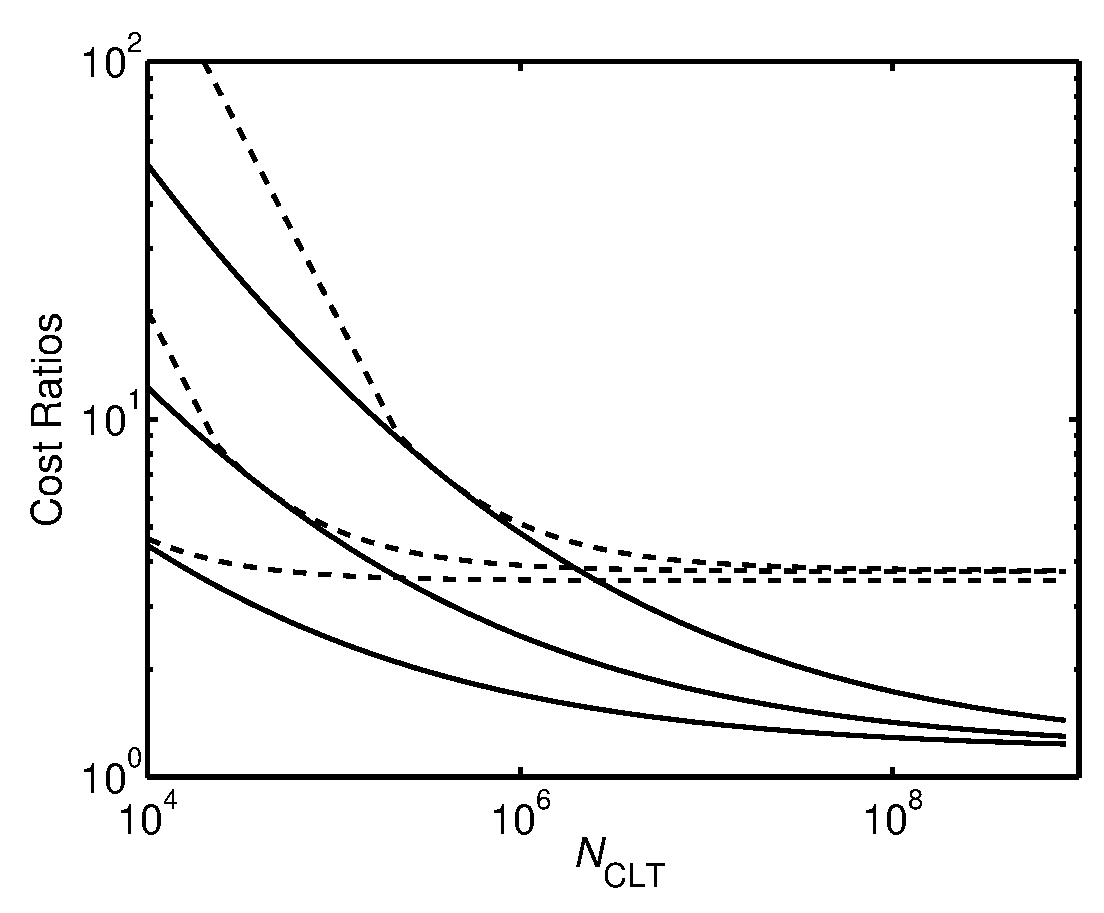
\includegraphics[width=2.1in]{MCSampleSizes} \\
% switch to kurtmaxfig.eps if not using pdflatex
(a)
\end{minipage}
\quad 
\begin{minipage}{2.3in}\centering
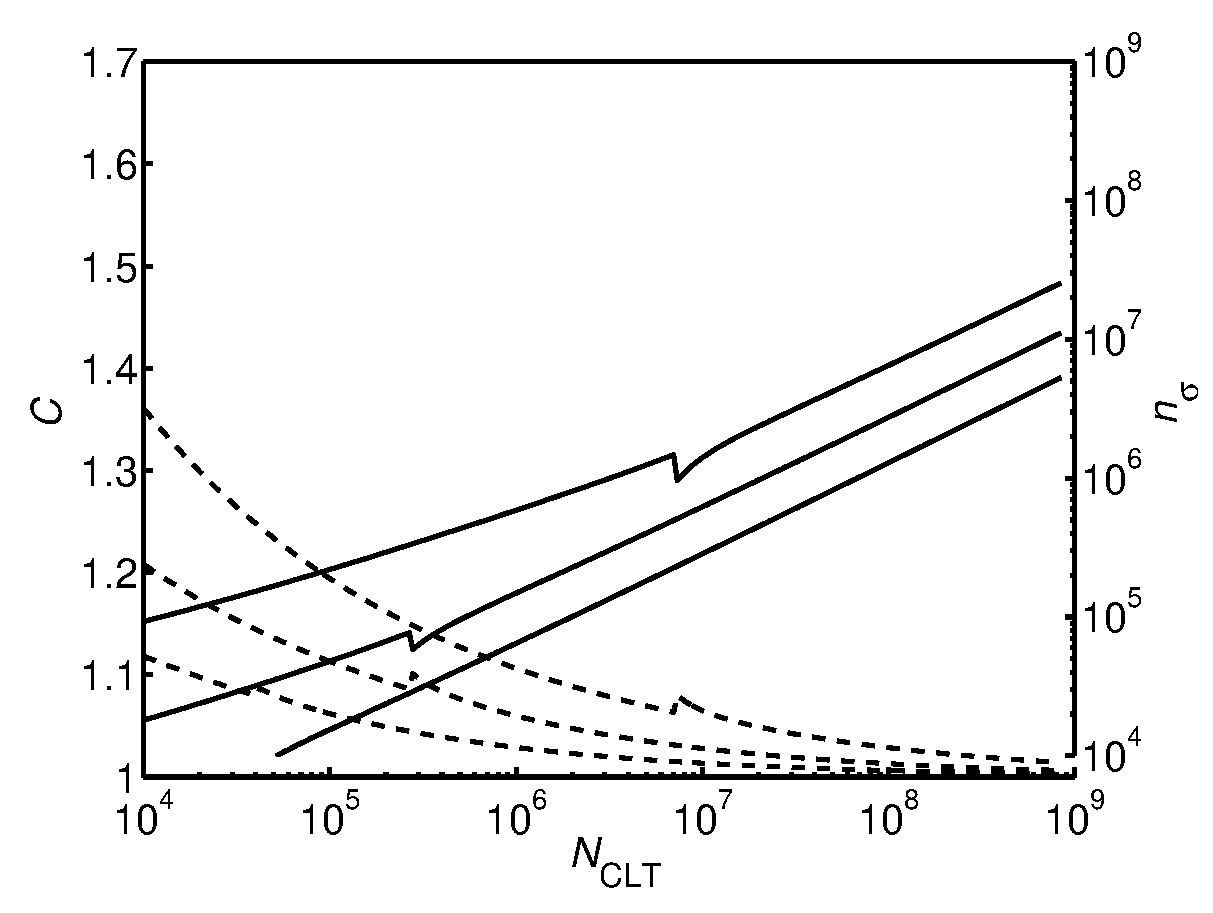
\includegraphics[width=2.3in]{MCnsigmafudge}\\
(b)
\end{minipage}
\caption{(a) The ratio of $\cost(\aMC,\varepsilon,0.01,0.01, \tkappa_{\max}, \sigma)$ to $N_{\mathrm{CLT}}(\varepsilon,\sigma,0.01)$, as defined in \eqref{kappamaxdef}; (b) comparison of sample sizes $ N_G(0.01,\alpha)$, $N_C(0.01,\alpha)$, and $N_B(0.01,\alpha,\kappa_{\max}^{3/4}(\alpha,1000,1.5))$.\label{Costfig}}
\end{figure}

Figure \ref{Costfig}a shows the ratio of $N_{\rm{up}}(\varepsilon,0.01,0.01, \tkappa_{\max}, \sigma)$ to $N_{\mathrm{CLT}}(\varepsilon,\sigma,0.01)$ for a range of $\sigma/\varepsilon$ ratios for $\tkappa_{\max}=10,100$, and $1000$.  Note that $N_{\mathrm{CLT}}(\varepsilon,\sigma,0.01)$ and $\sigma/\varepsilon$ are equivalent to each other. The solid curves denote the case of choosing $n_\sigma$ and $\fudge$ varying with $\sigma/\varepsilon$ to minimize $N_{\rm{up}}$.  Figure \ref{Costfig}b displays the optimal values of $n_\sigma$ (solid) and $\fudge$ (dashed).  In both figures, higher curves correspond to higher values of $\tkappa_{\max}$. Here $N_{\mathrm{CLT}}$ denotes the ideal cost if one knew the variance of $Y$ a priori and knew that the distribution of the sample mean was close to Gaussian. The ratio is the penalty for having a guaranteed fixed-width confidence interval in the absence of this knowledge.  For smaller values of $N_{\mathrm{CLT}}$ (or  $\sigma/\varepsilon$) the cost of Algorithm \ref{twostagealgo} can be rather large.  However the absolute penalty is somewhat less because the total number of samples needed is not much.  For larger $N_{\mathrm{CLT}}$ (or $\sigma/\varepsilon$) the ratio approaches somewhat less than $1.5$.

The dashed curves in Figure \ref{Costfig}a show the ratio of $N_{\rm{up}}(\varepsilon,0.01,0.01, \tkappa_{\max}, \sigma)$ to $N_{\mathrm{CLT}}(\varepsilon,\sigma,0.01)$, but this time with $n_\sigma=1000\tkappa_{\max}$, which corresponds to $\fudge \approx 1.2$. While the ratio is large for small $N_{\mathrm{CLT}}$ (or  $\sigma/\varepsilon$), it approaches less than $4$ for large $N_{\mathrm{CLT}}$ (or  $\sigma/\varepsilon$).

Although $n_\sigma$ can be as small as $2$, it should be chosen much larger.  Our suggestion is to choose $\fudge$ around $1.2$--$1.5$, and then choose $n_\sigma$ as large as needed to ensure that $\tkappa_{\max}$ is as large as desired.
ordinarily be larger.  

\section{Numerical Examples with Algorighm \ref{twostagealgo}} \label{numerexsec}

\subsection{Illustrative Univariate Examples of Automatic Algorithms}

Several commonly used software packages have automatic algorithms for integrating functions of a single variable.  These include 
\begin{itemize} 

\item {\tt quad} in MATLAB \citep{MAT7.12}, adaptive Simpson's rule based on {\tt adaptsim} by \cite{GanGau00a},

\item {\tt quadgk} in MATLAB \citep{MAT7.12}, adaptive Gauss-Kronrod quadrature based on {\tt quadva} by \cite{Sha08a}, and

\item the {\tt chebfun} \citep{TrefEtal12} toolbox for MATLAB \citep{MAT7.12}, which approximates integrals by integrating interpolatory Chebychev polynomial series for the integrands.

%\item {\tt NIntegrate} in Mathematica \citep{Mat8a}, which uses a number of adaptive rules for one dimensional integrals, 

\end{itemize}

For the first three of these automatic algorithms one can easily probe where they sample the integrand, feed the algorithms zero values, and then construct fooling functions for which the automatic algorithms will return a zero value for the integral.  Figure \ref{foolfunfig} displays these fooling functions for the problem $\mu=\int_0^1 f(x) \, \dif x$ for these three algorithms. Each of these algorithms is asked to provide an answer with an absolute error no greater than $10^{-14}$, but in fact the the absolute error is $1$ for these fooling functions.  The algorithms {\tt quad} and {\tt chebfun} sample only about a dozen points before concluding that the function is zero, whereas the algorithm {\tt quadgk} samples a much larger number of points (only those between $0$ and $0.01$ are shown in the plot). 

\begin{figure}
\centering
\begin{minipage}{3.7cm} \centering 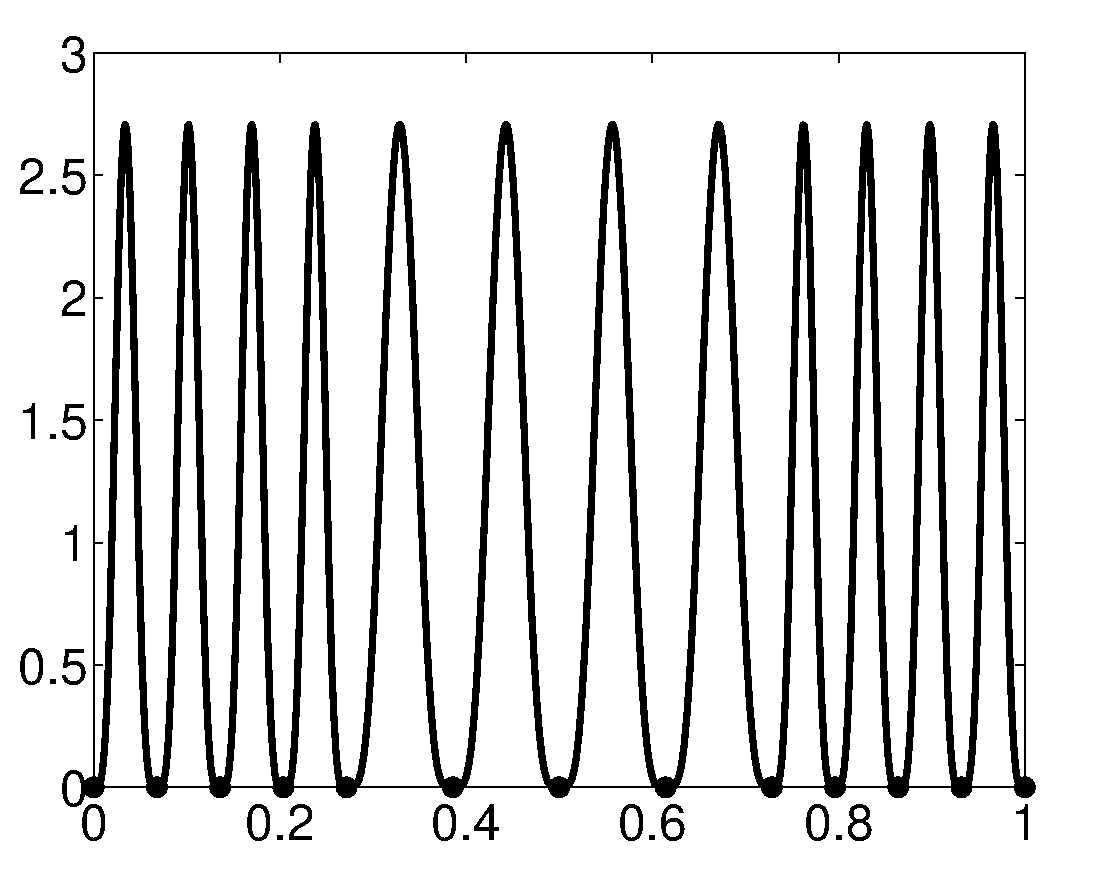
\includegraphics[width=3.7cm]{Foolquadbw.eps} \\ {\tt quad} \end{minipage}
\begin{minipage}{3.7cm} \centering 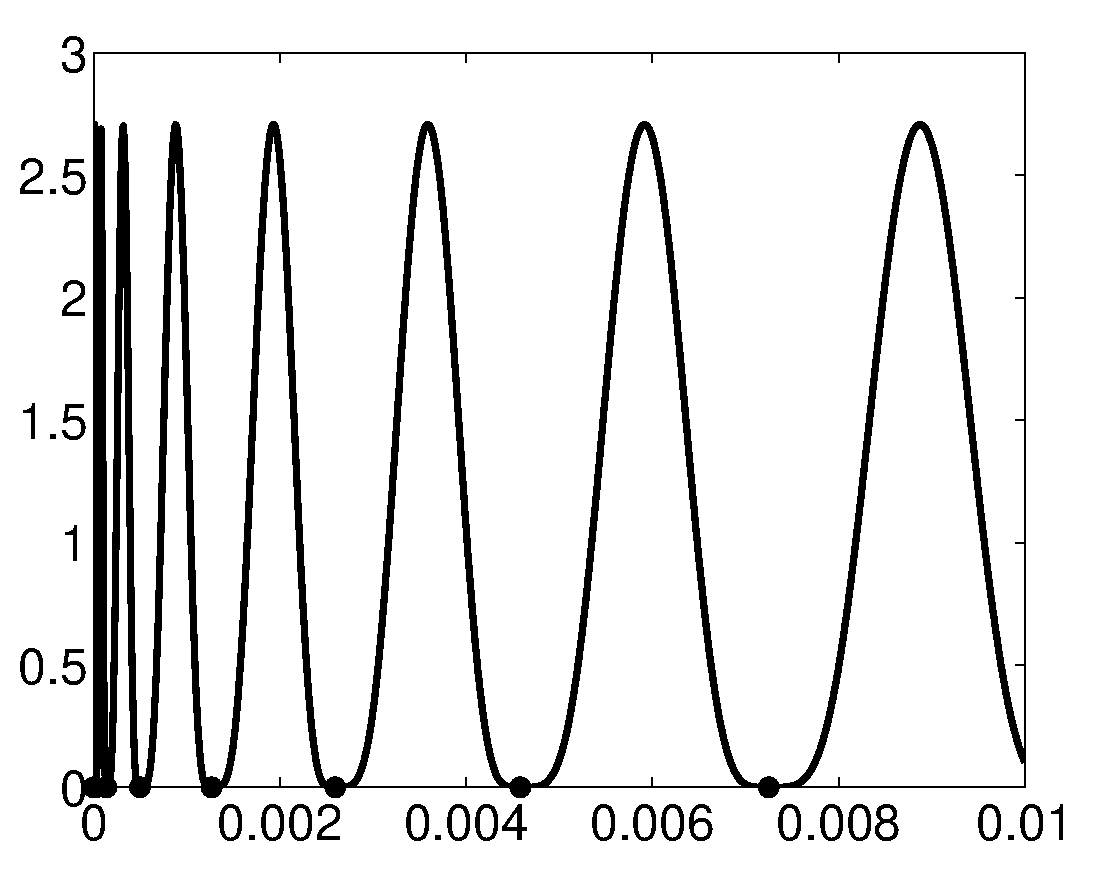
\includegraphics[width=3.7cm]{Foolquadgkbw.eps} \\ {\tt quadgk} \end{minipage}
\begin{minipage}{3.7cm} \centering 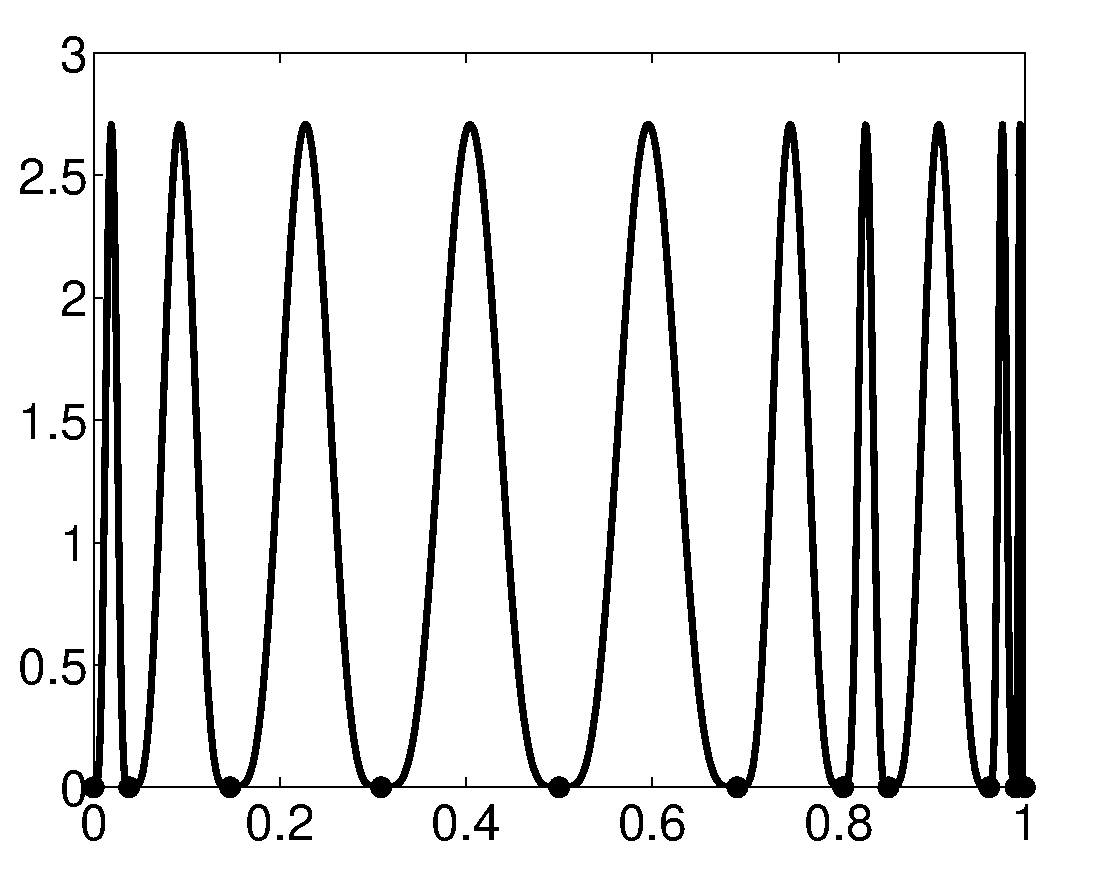
\includegraphics[width=3.7cm]{Foolchebintbw.eps} \\ {\tt chebfun} \end{minipage}
\caption{Plots of fooling functions, $f$, with $\mu=\int_0^1 f(x) \, \dif x=1$, but for which the corresponding algorithms return values of $\hmu=0$. \label{foolfunfig}}
\end{figure}


Accuracy and timing results have been recorded for the test function
\begin{equation} \label{GaussianTestFun}
f(\vx)=a_0 + b_0\prod_{j=1}^d\left[ 1 +b_j \exp \left(-\frac{(x_j-h_j)^2}{c_j^2}\right) \right].
\end{equation}
Here $\vx$ is a $d$ dimensional vector, and the $b_j$, $c_j$, and $h_j$ are parameters.  For Figure \ref{GaussianTestFunFig} shows the results of different algorithms being used to integrate $500$ different instances of $f$.  For each instance of $f$, the parameters are chosen as follows:
\begin{itemize} 
\item $b_j \in [0.1,10]$ with $\log(b_j)$ being i.i.d.\ uniform, $j=1, \ldots, d$,
\item $c_j \in [10^{-6},1]$ with $\log(c_j)$ being i.i.d.\ uniform, $j=1, \ldots, d$,
\item $h_j \in [0,1]$ with $h_j$ being i.i.d.\ uniform, $j=1, \ldots, d$,
\item $b_0$ chosen in terms of the $b_j$, $c_j$, and $h_j$ in order to make $\sigma^2(f) \in [10^{-2}, 10^2]$, with $\log(\sigma(f))$ being i.i.d.\ uniform for each instance, and
\item $a_0$ in terms of chosen in terms of the $b_j$, $c_j$, and $h_j$ to make $\mu(f)=1$.
\end{itemize}
These ranges of parameters are chosen so that the algorithms being tested fail to meet the error tolerance a significant number of times.

\begin{figure}
\centering
\begin{minipage}{5.7cm} \centering 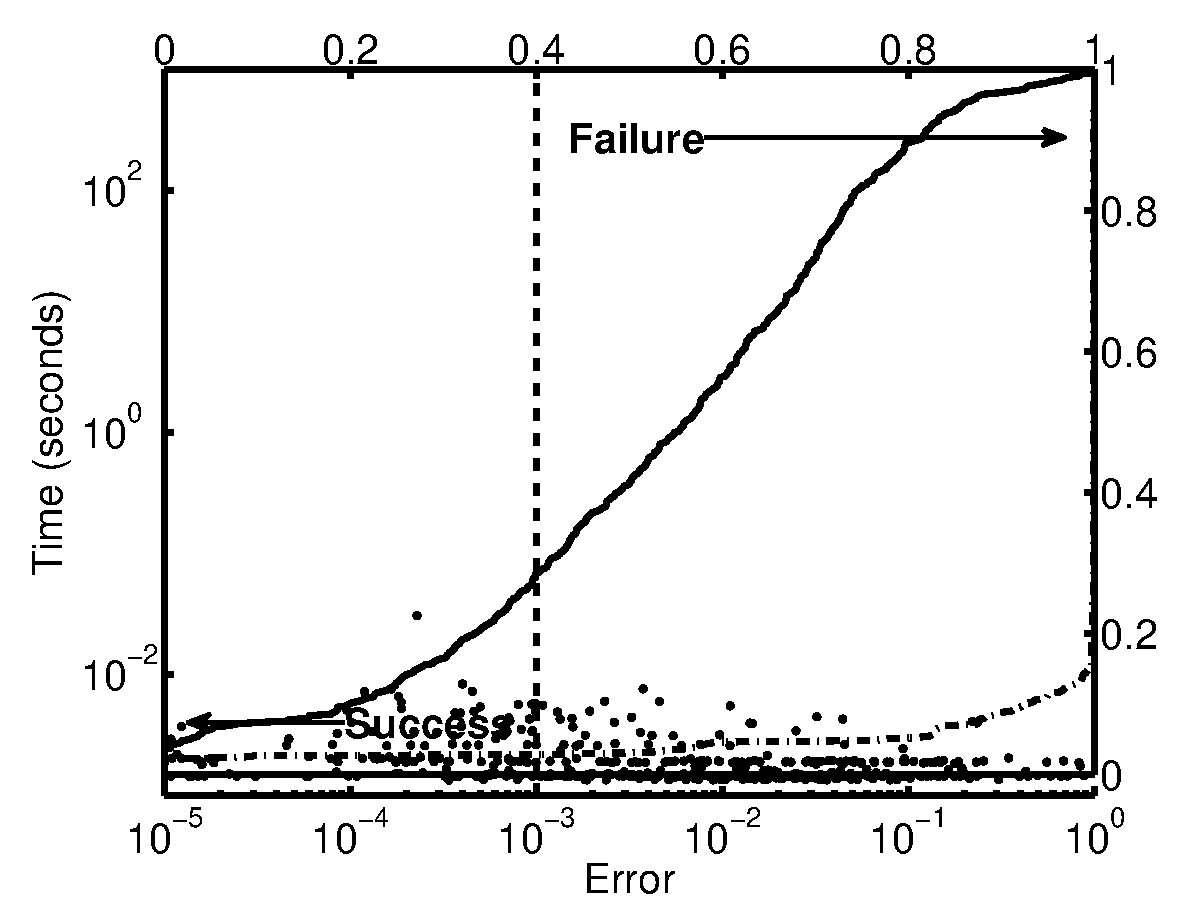
\includegraphics[width=5.7cm]{gaussiand=1quadErrTime.eps} \\ {\tt quad} \end{minipage}
\begin{minipage}{5.7cm} \centering 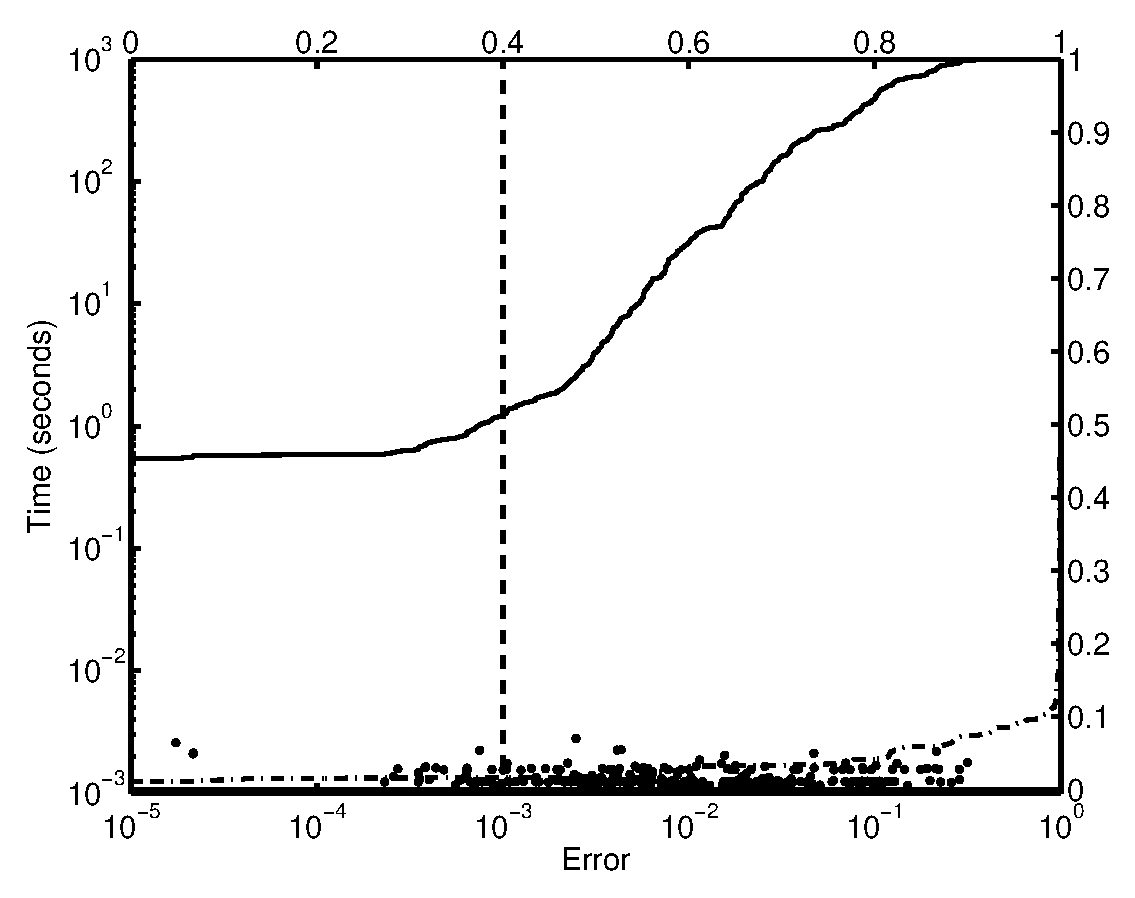
\includegraphics[width=5.7cm]{gaussiand=1quadgkErrTime.eps} \\ {\tt quadgk} \end{minipage}
\begin{minipage}{5.7cm} \centering 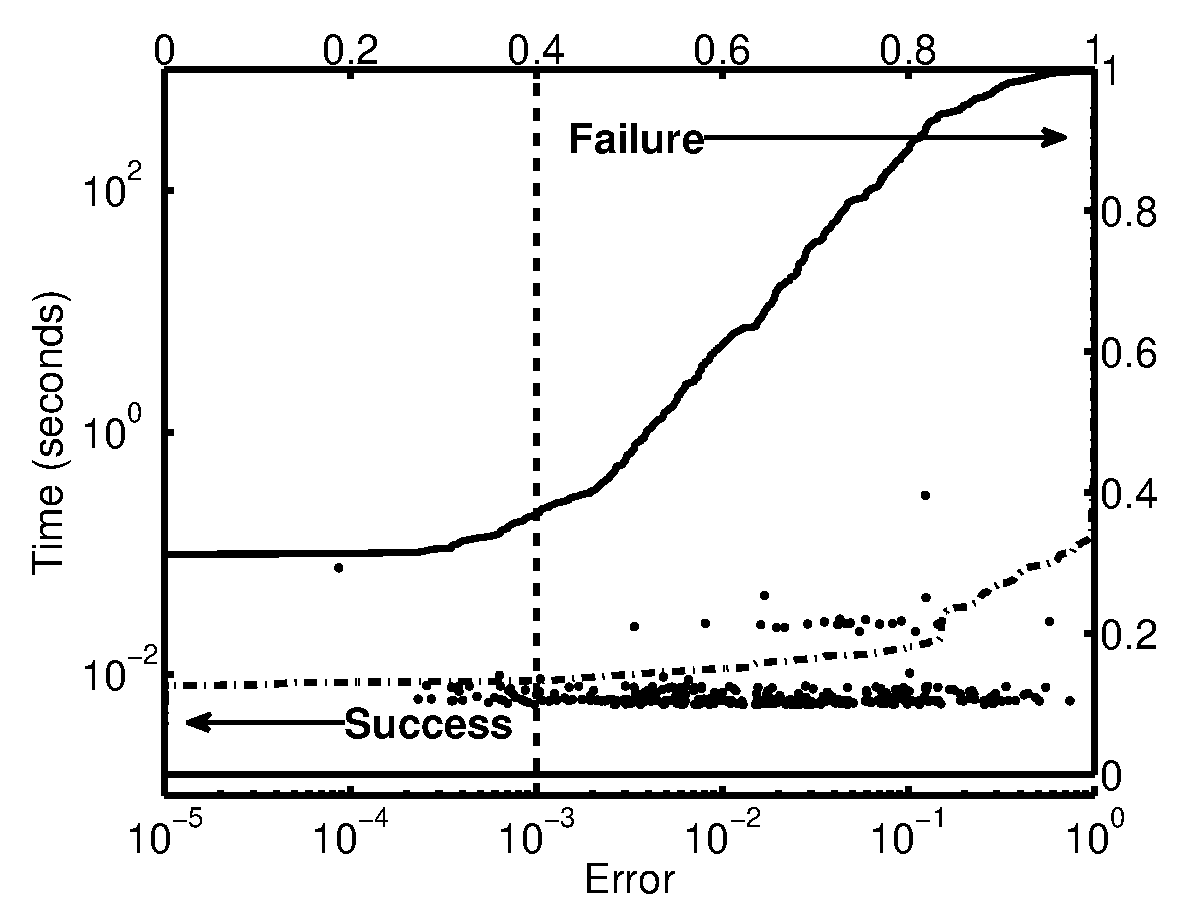
\includegraphics[width=5.7cm]{gaussiand=1chebfunErrTime.eps} \\ {\tt chebfun} \end{minipage}
\begin{minipage}{5.7cm} \centering 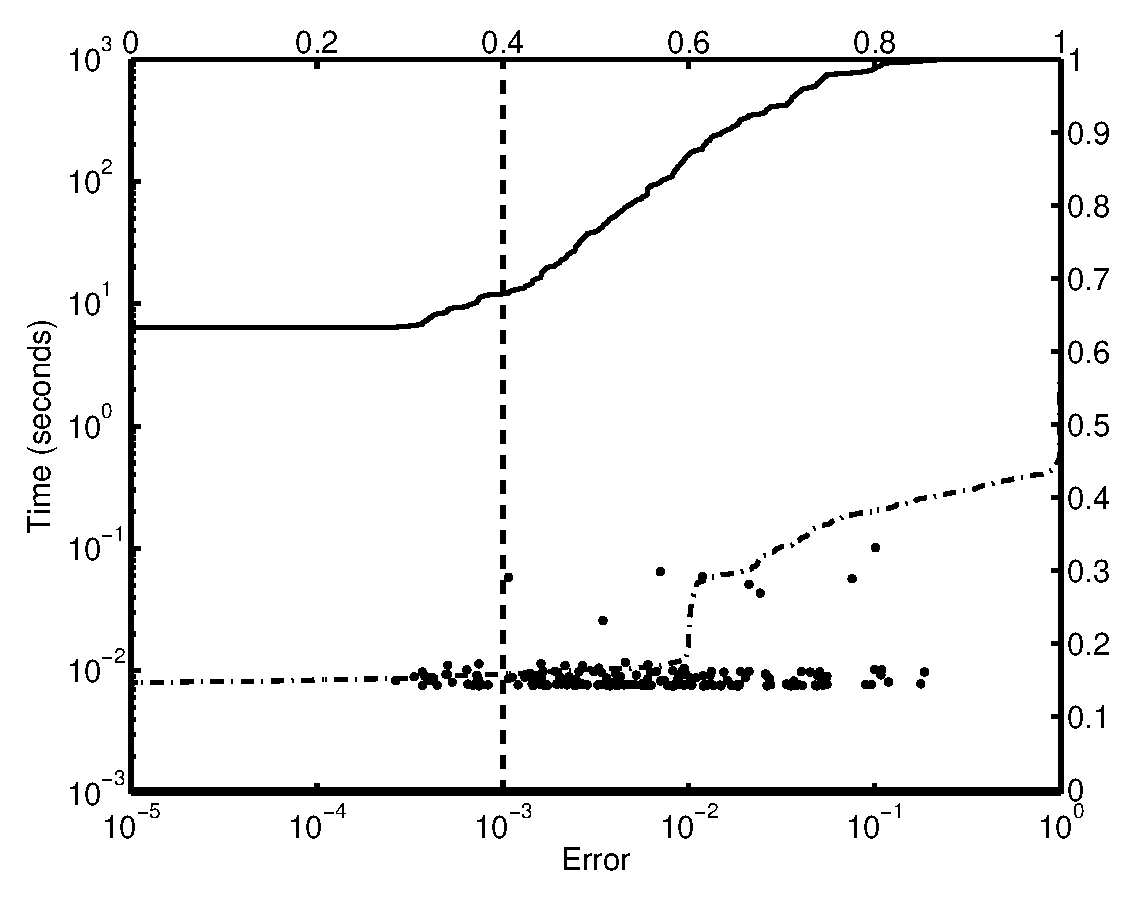
\includegraphics[width=5.7cm]{gaussiand=1chebfunheavyErrTime.eps} \\ {\tt chebfun}  (heavy duty) \end{minipage}
\begin{minipage}{5.7cm} \centering 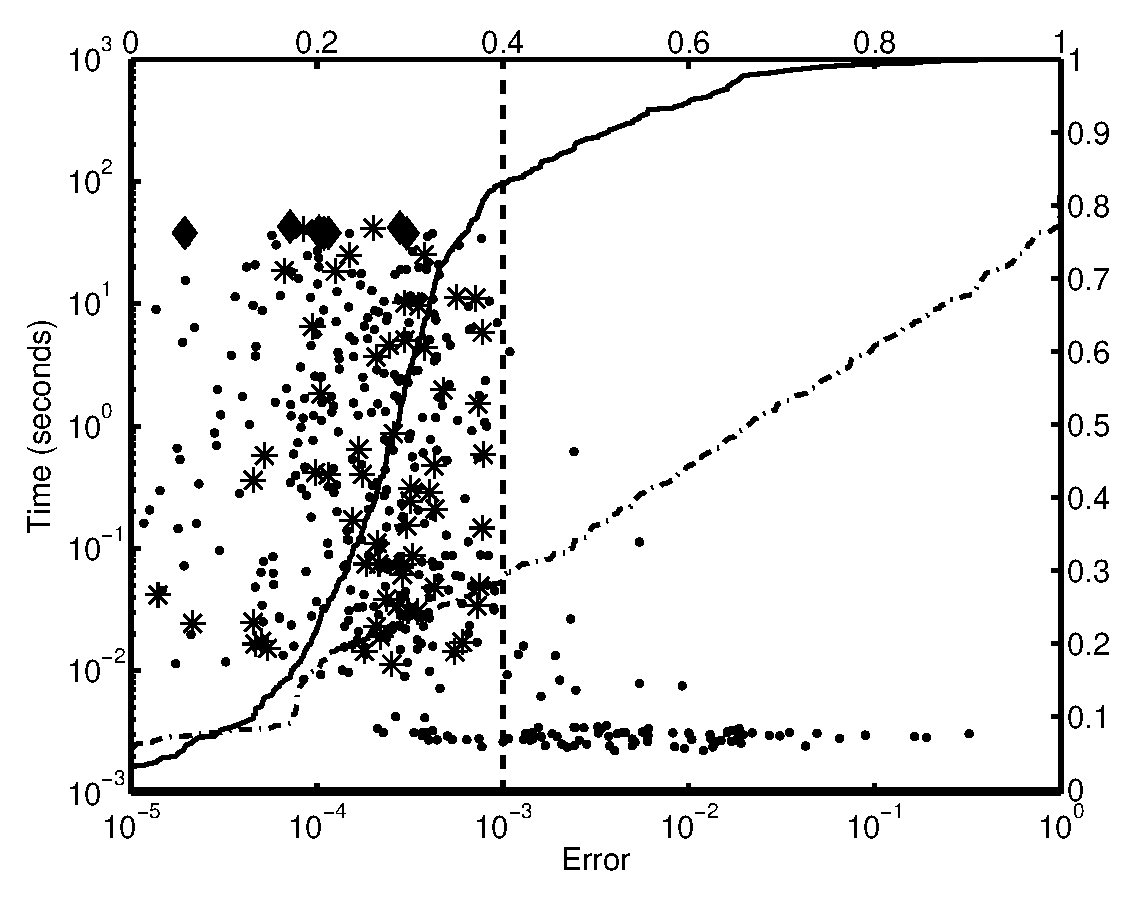
\includegraphics[width=5.7cm]{gaussiand=1iidErrTime.eps} \\ Algorithm \ref{twostagealgo}  \end{minipage}
\begin{minipage}{5.7cm} \centering 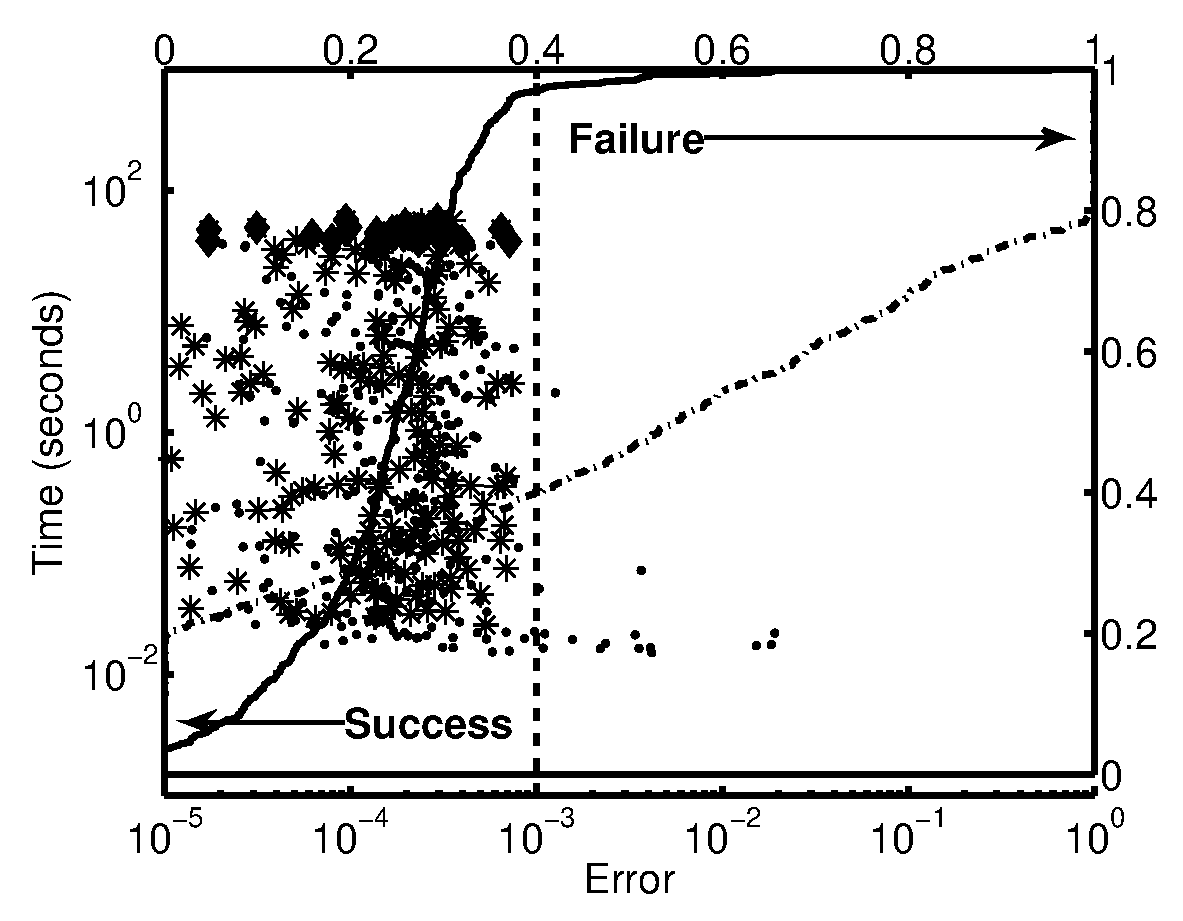
\includegraphics[width=5.7cm]{gaussiand=1iidheavyErrTime.eps} \\ Algorithm \ref{twostagealgo} (heavy duty)\end{minipage}
\begin{minipage}{5.7cm} \centering 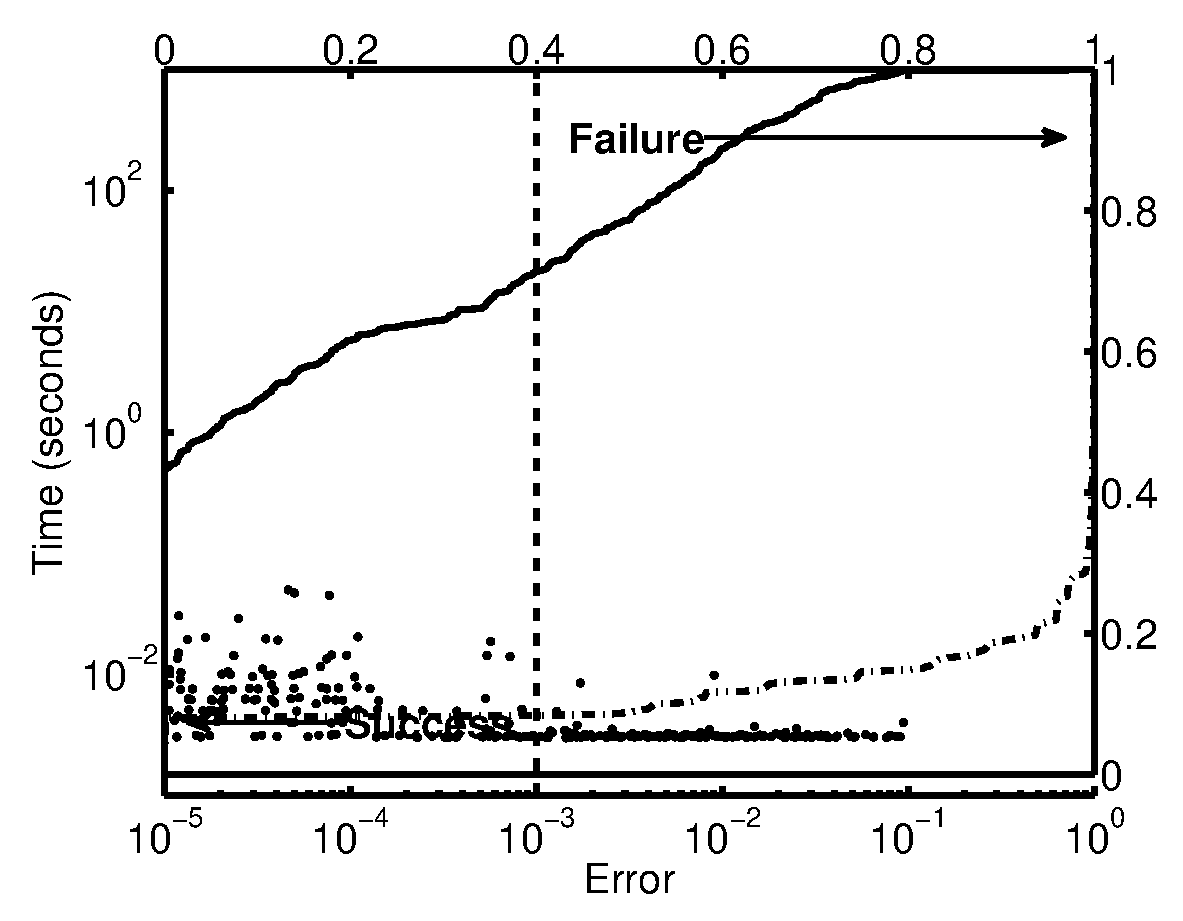
\includegraphics[width=5.7cm]{gaussiand=1SobolErrTime.eps} \\  Sobol'\end{minipage}
\begin{minipage}{5.7cm} \centering 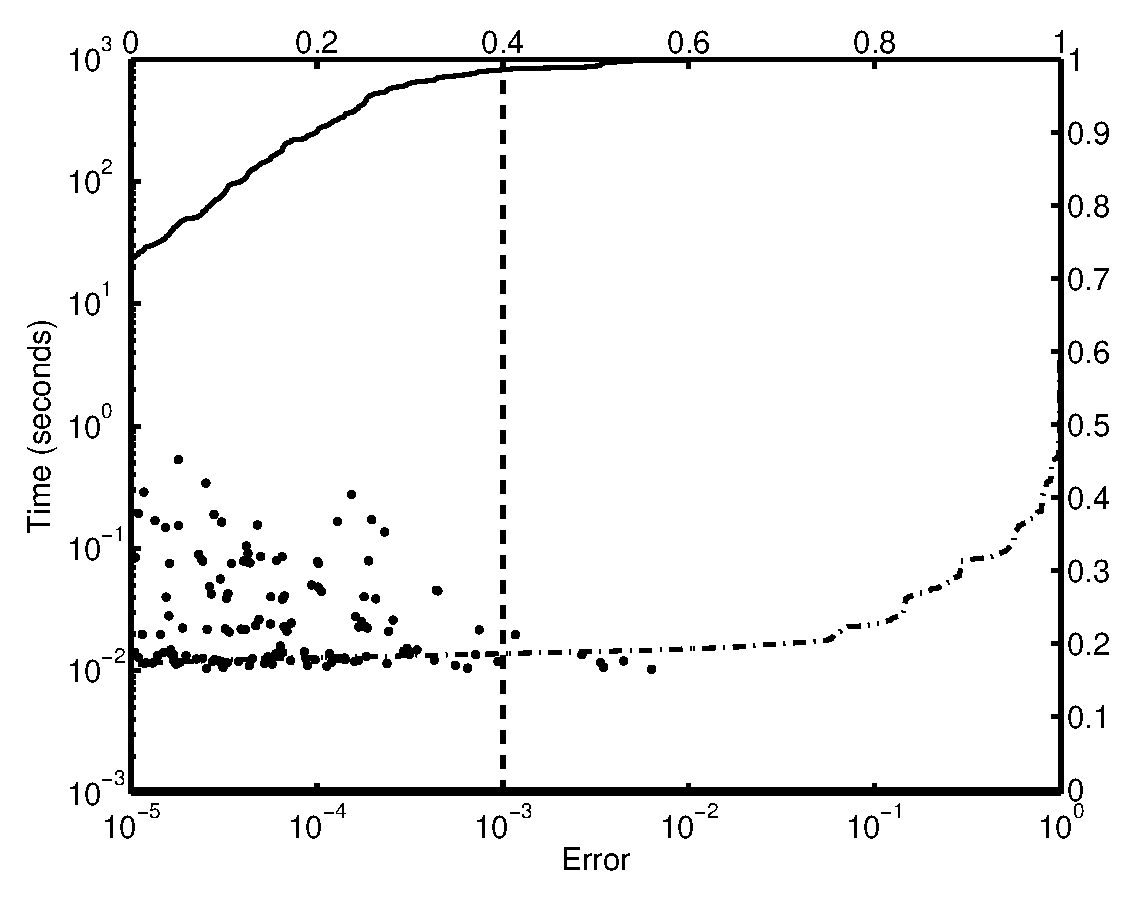
\includegraphics[width=5.7cm]{gaussiand=1SobolheavyErrTime.eps} \\ Sobol' heavy duty \end{minipage}
\caption{Execution times and errors for test function \eqref{GaussianTestFun} for $d=1$ and $\varepsilon=10^{-3}$, and a variety of parameters giving a range of $\sigma(f)$ and $\kappa(f)$. The solid line shows that cumulative distribution of actual errors, and the dot-dashed line shows the cumulative distribution of execution times.  For the Algorithm \ref{twostagealgo} the points labeled * are those for which the Theorem \ref{mainadaptthm} guarantees the error tolerance.\label{GaussianTestFunFig} }
\end{figure}

These $500$ random constructions of $f$ with $d=1$ are integrated over $[0,1]$ with $\rho=1$ (the uniform density function), using {\tt quad},  {\tt quadgk}, {\tt chebfun}, and Algorithm \ref{twostagealgo}, and an automatic quasi-Monte Carlo algorithm that uses scrambled Sobol' sampling \citep{Owe95,Owe96,Owe97,Mat98,HonHic00a,DicPil10a} and quasi-standard error \citep{Hal05a,Owe06a} to determine the sample size.  We do not yet have a theorem providing sufficient conditions under which this quasi-Monte Carlo algorithm is guaranteed to provide the answer within the specified error tolerance, and so we do not describe this algorithm in detail.  

For all but {\tt chebfun}, the specified absolute error tolerance is $\epsilon=0.001$.  The algorithm {\tt chebfun} attempts to do all calculations to near machine precision.  The observed error and execution times are plotted in Figure \ref{GaussianTestFunFig}.  Whereas {\tt chebfun} uses a minimum of $2^3+1=9$ function values, the figure labeled ``{\tt chebfun} (heavy duty)'' displays the results of requiring chebfun to use at least $2^{10}+1=1025$ function values.  Algorithm \ref{twostagealgo} takes $\alpha=0.01$, and $\fudge=1.5$.  For the plot on the left, $n_\sigma=2^{10}=1024$, which corresponds to  $\tkappa_{\max}=2.59$.  For the heavy duty plot on the right, $n_\sigma=2^{17}=131\ 072$, which corresponds to  $\kappa_{\max}=205$.  The same initial sample sizes are used for the Sobol' sampling algorithm.

Figure \ref{GaussianTestFunFig} shows that {\tt quad} and {\tt quadgk} are quite fast, nearly always providing an answer in less that $0.01$ seconds.  Unfortunately, they successfully meet the error tolerance only about $30\%$ of the time for {\tt quad} and $50$--$60\%$ of the time for {\tt quadgk}.  The difficult cases are those where $c_1$ is quite small, and these algorithms miss the sharp peak.  The performance of {\tt chebfun} is similar to that of {\tt quad} and {\tt quadgk}.  The heavy duty version of  {\tt chebfun} fares somewhat better.  

In the plots for Algorithm \ref{twostagealgo} those points where the integrands satisfy $\tkappa(f) \le \tkappa_{\max}$ are labeled *, and all such points fall within the prescribed error tolerance.  For Algorithm \ref{twostagealgo} (heavy duty) $\kappa_{\max}$ is larger, so there are more points for which the guarantee holds.  Those points labeled with a dot, are those for which $\tkappa(f) > \tkappa_{\max}$, and so no guarantee holds. The points labeled with a diamond are those for which Algorithm \ref{twostagealgo} attempts to exceed the cost budget that we set, i.e., it wants to choose $n$ such that $(n_{\sigma}+n)d > N_{\max}=10^9$. Algorithm \ref{twostagealgo} performs somewhat more robustly than {\tt quad}, {\tt quadgk}, and {\tt chebfun}, because it requires only a low degree of smoothness and takes a fairly large minimum sample.  The more important point is that Algorithm \ref{twostagealgo} has a guarantee, where to our knowledge, the other routines do not.

From Figure \ref{GaussianTestFunFig}, the Sobol' sampling algorithm is more reliable and takes less time than Algorithm \ref{twostagealgo}.  This is due primarily to the fact that in dimension one, Sobol' sampling is equivalent to stratified sampling, where the points are more evenly spread.

Figure \ref{GaussianTestFunHDFig} repeats the simulation shown in Figure \ref{GaussianTestFunFig} for the same test function \eqref{GaussianTestFun}, but now with $d=2, \ldots, 8$ chosen randomly and uniformly.  For this case the univariate integration algorithms are inapplicable, but the two multidimensional routines can be used.  There are more cases where the Algorithm \ref{twostagealgo} tries to exceed the maximum sample size allowed, but the behavior seen for $d=1$ still generally apply.  

\begin{figure}
\centering
\begin{minipage}{5.7cm} \centering 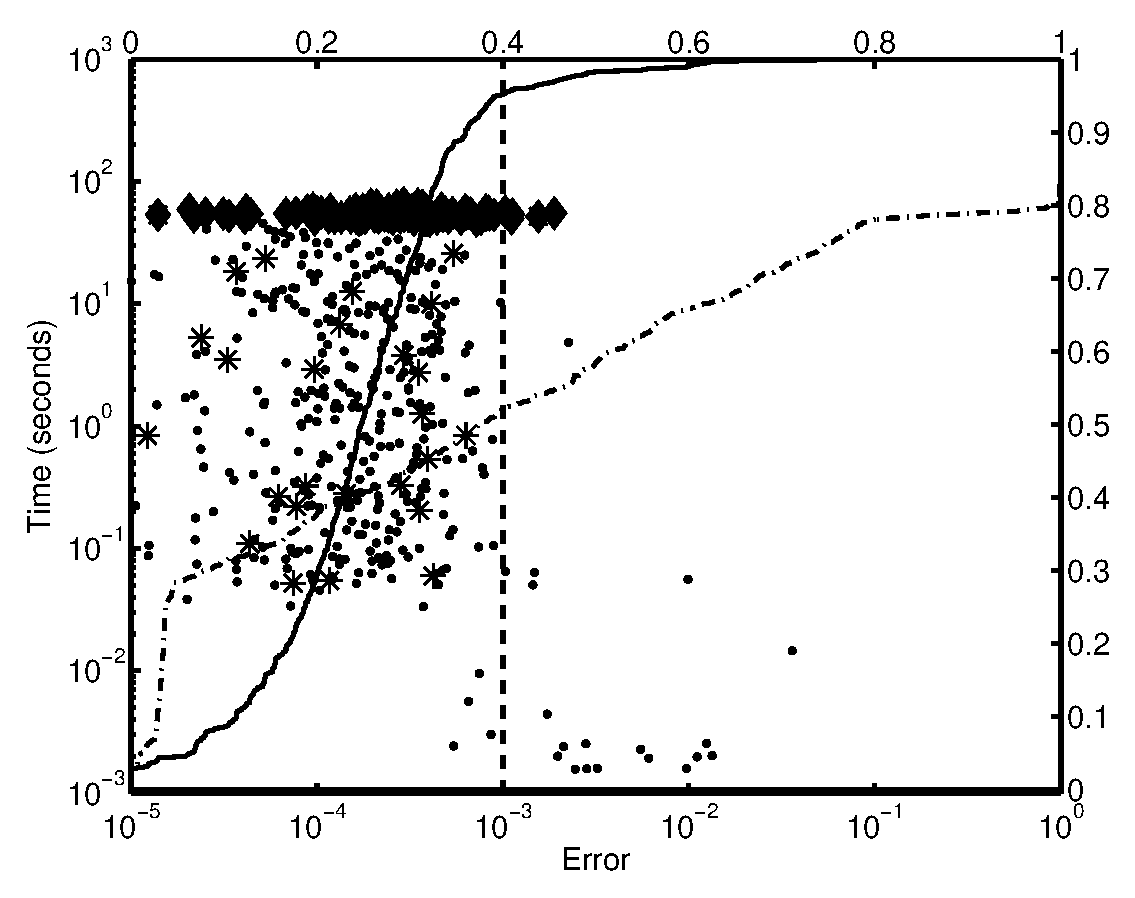
\includegraphics[width=5.7cm]{gaussiand=6iidErrTime.eps} \\ {\tt cubMC} i.i.d. \end{minipage}
\begin{minipage}{5.7cm} \centering 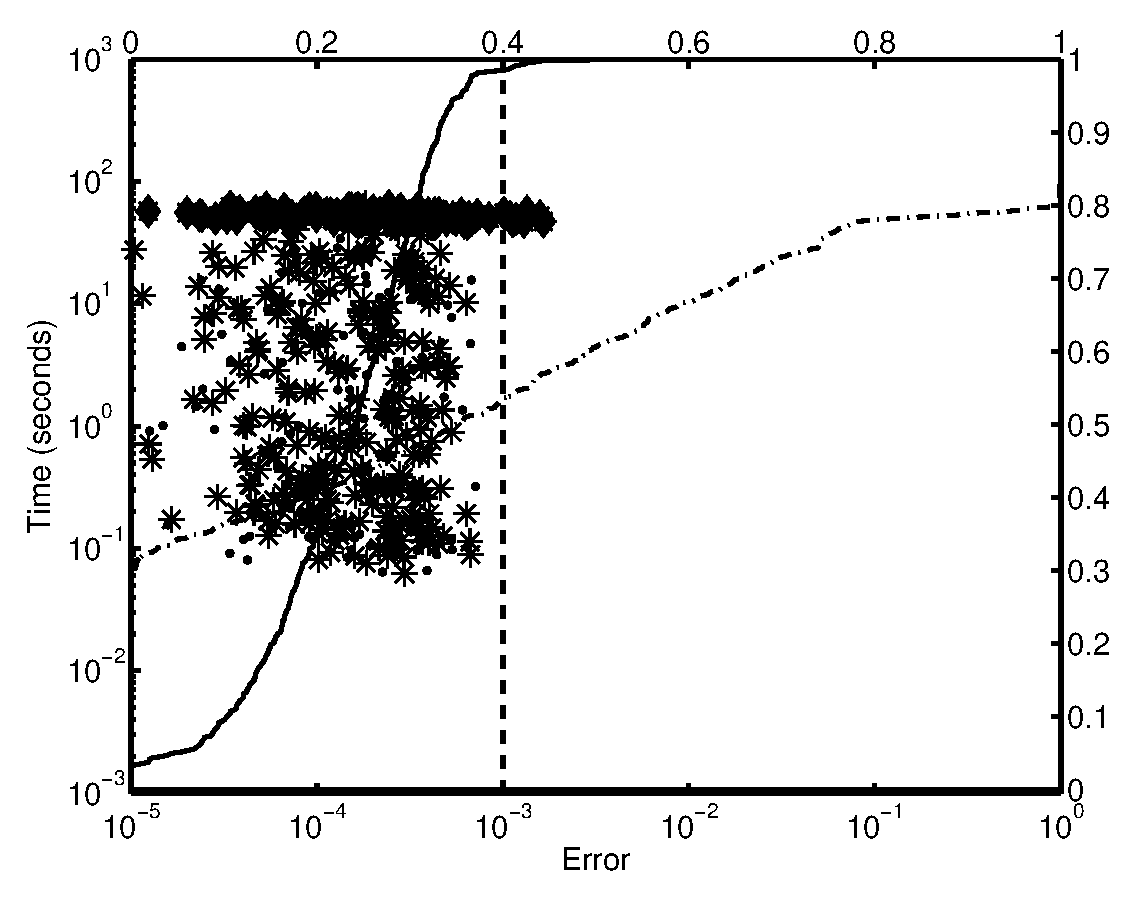
\includegraphics[width=5.7cm]{gaussiand=6iidheavyErrTime.eps} \\ {\tt cubMC} i.i.d heavy duty \end{minipage}
\begin{minipage}{5.7cm} \centering 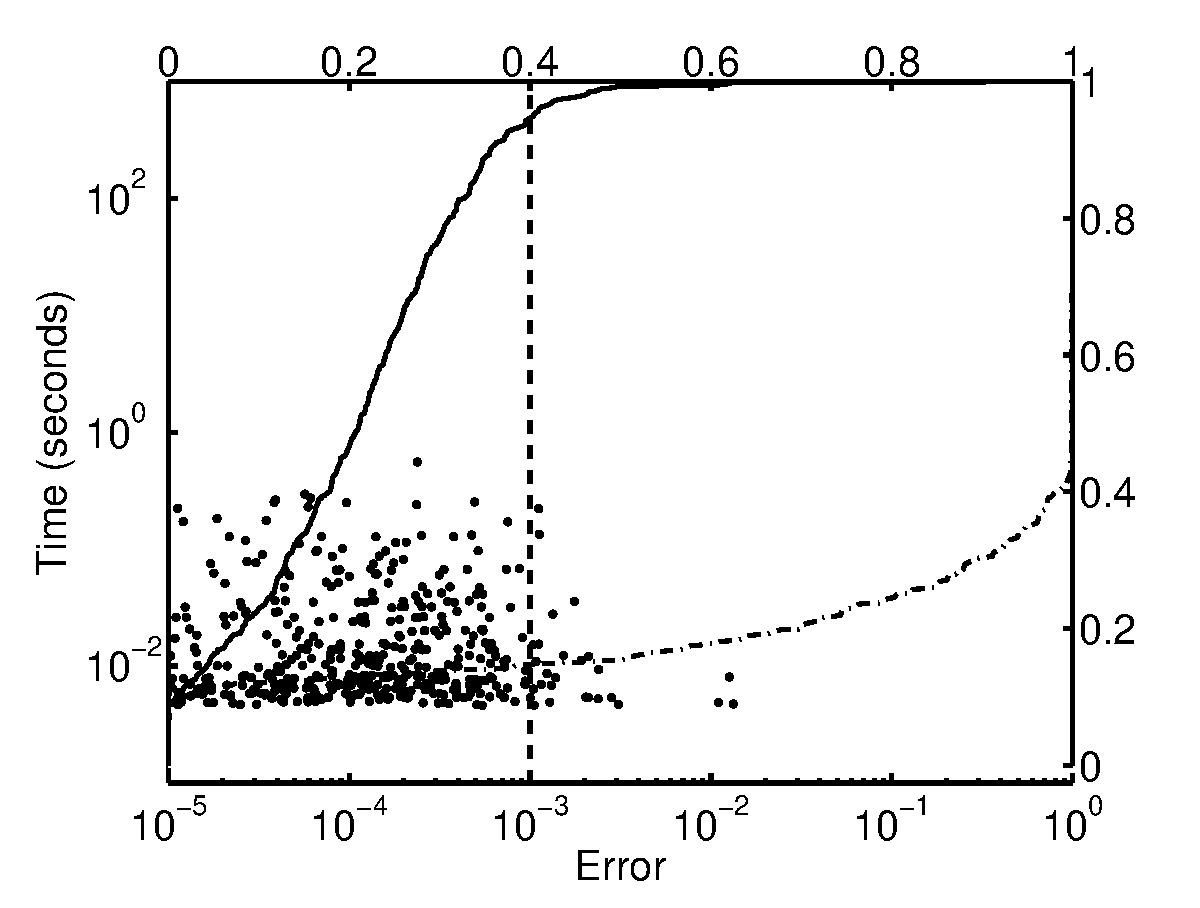
\includegraphics[width=5.7cm]{gaussiand=6SobolErrTime.eps} \\ {\tt cubMC} Sobol' \end{minipage}
\begin{minipage}{5.7cm} \centering 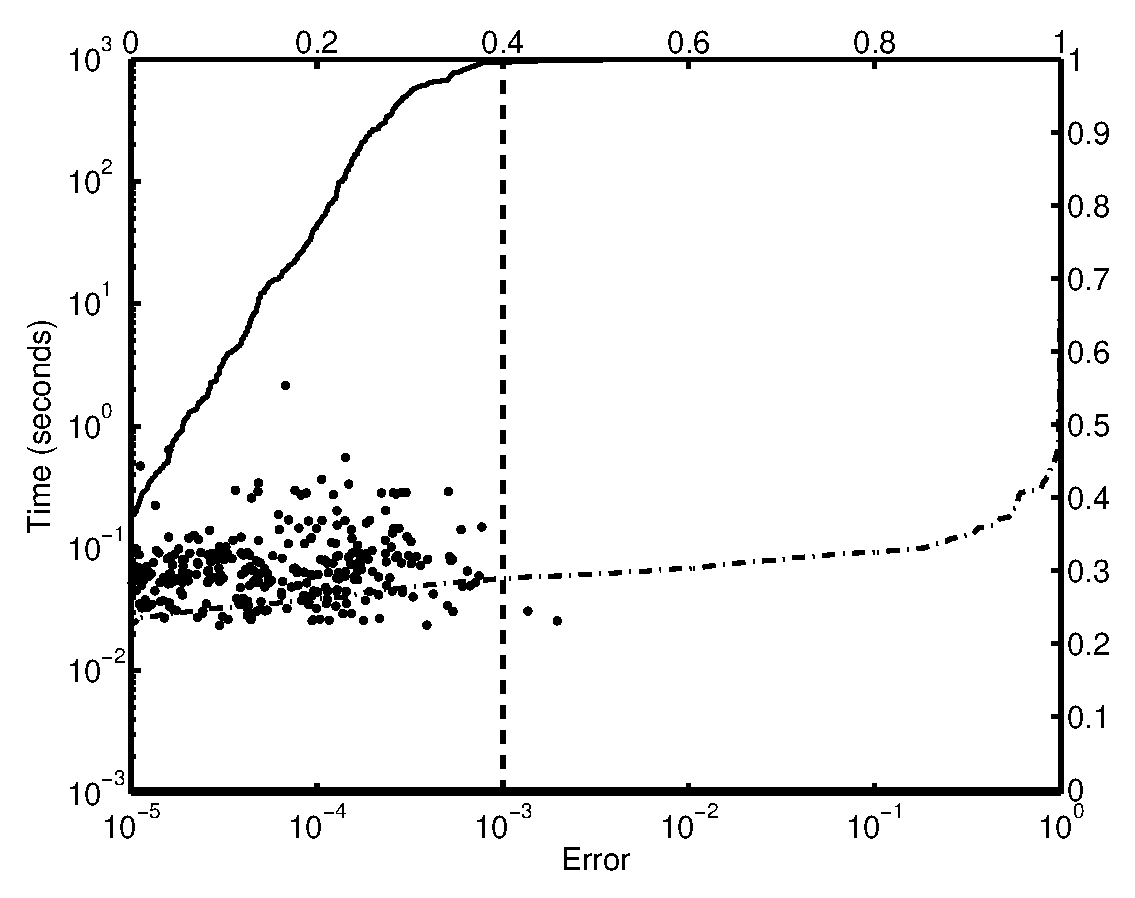
\includegraphics[width=5.7cm]{gaussiand=6SobolheavyErrTime.eps} \\ {\tt cubMC} Sobol' heavy duty \end{minipage}
\caption{Execution times and errors for test function \eqref{GaussianTestFun} for $d=2, \ldots, 8$ and $\varepsilon=10^{-3}$, with the rest of the parameters as in Figure \ref{GaussianTestFunFig}.\label{GaussianTestFunHDFig}}
\end{figure}

{\bf We will put one more finance example here.}

\section{A General Error Criterion} \label{relerrsec}

In many practical situations, one needs to approximate the integral with a certain relative accuracy.  For example, one wants an answer that is correct to three significant digits.  In this case, given a tolerance, $\varepsilon$, and a significance level $\alpha$, with $\varepsilon, \alpha \in (0, 1)$, one seeks a random $\tmu$ such that 
\begin{equation*} \label{relerrcrit}
\Prob\left[\abs{\frac{\tmu-\mu}{\mu}} \le \varepsilon \right] \geq 1-\alpha.
\end{equation*}
A more general form of this criterion would be
\begin{equation} \label{genrelerrcrit}
\Prob\left[\frac{\abs{\tmu-\mu}} {1-\theta + \theta\abs{\mu}} \le \varepsilon \right] \geq 1-\alpha.
\end{equation}
for some fixed $\theta \in [0,1]$, where $\theta=0$ corresponds to absolute error, and $\theta = 1$ corresponds to relative error.  Clearly, one must have $(1-\theta) + \abs{\mu}\ne0$ for such a statement to be possible.  

If $\varepsilon_{A} \ge 0$ is an absolute error tolerance, and $\varepsilon_{R} \ge 0$ is a relative error tolerance, then letting 
\[
\varepsilon = \frac{\varepsilon_{A}\varepsilon_{R}}{\theta \varepsilon_{A} + (1-\theta) \varepsilon_{R}},
\]
it follows that for all $\theta \in [0,1]$,
\[
[1-\theta + \theta \abs{\mu}]\varepsilon = (1-\gamma)\varepsilon_{A} + \gamma \varepsilon_{R} \abs{\mu} \le \max(\varepsilon_{A},\varepsilon_{R} \abs{\mu}),
\]
where
\[
\gamma = \frac{\theta \varepsilon_{A}}{\theta \varepsilon_{A} + (1-\theta) \varepsilon_{R}} \in [0,1].
\]
Thus, error criterion  \eqref{genrelerrcrit} implies that one has satisfied either an absolute or a relative error criterion, 
\[
\Prob\left[\frac{\abs{\tmu-\mu}} {1-\theta + \theta\abs{\mu}} \le \varepsilon \right] \geq 1-\alpha \implies \Prob\left[\abs{\tmu-\mu} \le \varepsilon_A \text{ or } \abs{\tmu-\mu} \le \abs{\mu}\varepsilon_R \right] \geq 1-\alpha.
\]
A value of $\gamma$ close to zero implies a preference to fulfill the absolute error criterion while a value of $\gamma$ close to one implies a preference to fulfill the relative error criterion.

Obtaining a confidence interval of the form \eqref{genrelerrcrit}, proceeds in three stages: i) obtaining an upper bound on $\sigma^2$, ii) obtaining a lower bound on $1-\theta + \theta\abs{\mu}$, and iii) then using these to obtain \eqref{genrelerrcrit}.  What differs from the absolute error case is step ii).  For this step it is noted that
\begin{multline} \label{relerrcritd}
\Prob\left[\abs{\hmu-\mu} \le \hvareps \right] \ge 1-\alpha \implies \Prob[\max(\abs{\hmu}-\hvareps,0) \le \abs{\mu} \le \abs{\hmu}+\hvareps] \ge 1-\alpha \\
\implies \Prob[1-\theta + \theta\max(\abs{\hmu}-\hvareps,0) \le 1-\theta + \theta\abs{\mu} \le 1-\theta + \theta(\abs{\hmu}+\hvareps)] \ge 1-\alpha.
\end{multline}
Although one might be happy the left side of this inequality being positive, if it is too much smaller than the right side, then one might be eventually expending too much extra work in step iii).  Thus, it makes sense to require 
\begin{gather*}
1-\theta + \theta\max(\abs{\hmu}-\hvareps,0) \ge \hdelta [1-\theta + \theta(\abs{\hmu}+\hvareps)] \\
\iff \hvareps = \begin{cases}
\displaystyle \frac{(1-\hdelta)(1-\theta)}{\hdelta \theta} -\abs{\hmu}, & 
\displaystyle 0 \le \abs{\hmu}  < \frac{(1-\hdelta)(1-\theta)}{2 \hdelta \theta},
 \\[2ex]
\displaystyle \frac{1-\hdelta}{1+\hdelta} \left[\frac{1-\theta}{\theta} +\abs{\hmu}\right], & 
\displaystyle \frac{(1-\hdelta)(1-\theta)}{2 \hdelta \theta} \le \abs{\hmu}  < \infty.
\end{cases}
\end{gather*}
This is done iteratively in the algorithm described in Theorem \ref{relerradaptthm} below.  One needs to prevent $\hvareps$ from becoming too small.  This means that $\hdelta$ should kept away from $1$, which means that the lower bound on $1-\theta + \theta\abs{\mu}$ is allowed to be somewhat smaller than the upper bound.  Preventing $\hvareps$ from becoming too small also means that $1-\theta + \abs{\hmu}$ cannot be too small. This may be unavoidable if one is interested in relative error $\theta=1$, and the true answer, $\mu$, is small.

Some notation is needed for this theorem.  For any fixed $\alpha \in (0,1)$, and $M>0$, define the inverse of the functions $N_C(\cdot,\alpha)$, $N_B(\cdot,\alpha,M)$, and $N_{CB}(\cdot,\alpha,M)$,
%\begin{subequations} \label{probadapterrcritBE}
\begin{gather*}\label{NCinv}
N_C^{-1}(n,\alpha) := \frac{1}{\sqrt{n \alpha}}, \\
\label{NBinv*}
N_B^{-1}(n,\alpha,M) := \min \left \{ b>0 : \Phi\left(-b \sqrt{n}  \right)+\frac{0.56M}{\sqrt{n}\left(1+ b\sqrt{n} \right)^{3}}
\le \frac{\alpha}{2} \right \}, \\
\label{NCBinv*}
N_{CB}^{-1}(n,\alpha,M) := \min(N_C^{-1}(n,\alpha),N_B^{-1}(n,\alpha,M)).
\end{gather*}
It then follows then by Chebychev's inequality and the Berry-Esseen Inequality (see \eqref{BEresult}) that 
\begin{equation*}
\Prob[\abs{\hmu_n -\mu}<\hvareps] \geq 1-\alpha, \quad \text{provided } \ f \in \cc_{\kappa_{\max}}, \text{ where }\hvareps=\sigma(f) N_{CB}^{-1}(n,\alpha,\kappa_{\max}^{3/4}), 
\end{equation*} 
%\end{subequations}
and $\sigma(f)=\sqrt{\var(f)}$ is the standard deviation of the integrand.  Given a significance level, $\alpha \in (0,1)$, let $\alpha_{\sigma}, \alpha_{\mu}, \alpha_1,  \alpha_2, \ldots$ be an infinite sequence of positive numbers all less than one, such that 
\begin{equation} \label{alphaseq}
(1-\alpha_{\sigma})(1-\alpha_{\mu})(1-\alpha_1)(1-\alpha_2) \cdots = 1-\alpha.
\end{equation}
For example, one might choose $\alpha_{\sigma},\alpha_{\mu},$ and $\halpha$ such that $(1-\alpha_{\sigma})(1-\alpha_{\mu})(1-\halpha)=1-\alpha$, and then 
\begin{equation} \label{alphaseqex}
\alpha_{i} = 1-(1-\halpha)^{(a-1)a^{-i}}, \ i\in \naturals, \quad \text{where} \  a \in (1,\infty).
\end{equation}

\begin{theorem} \label{relerradaptthm} Specify the following parameters defining the algorithm:
\begin{itemize}
\item sample size for variance estimation, $n_{\sigma} \in \naturals$,
\item initial sample size for mean estimation, $n_1 \in \naturals$,
\item variance inflation factor for variance estimation, $\fudge \in (1,\infty)$, 
\item factors for Step 2, $\hdelta, \delta, \tdelta \in (0,1)$, with $\delta < \tdelta$.
\item uncertainty tolerance, $\alpha\in (0,1)$, and a sequence $\alpha_{\sigma}, \alpha_{\mu}, \alpha_1,  \alpha_2, \ldots$ satisfying \eqref{alphaseq}, 
\item the parameter $\theta \in [0,1]$, used to define the general error criterion \eqref{genrelerrcrit}, and
\item the error tolerance, $\varepsilon >0$. 
\end{itemize} 
Let $\kappa_{\max}=\kappa_{\max}(n_{\sigma},\alpha_{\sigma},\fudge)$ as defined in \eqref{kappamaxdef}.  For any $f$ lying in the cone of functions with bounded kurtosis, $\cc_{\kappa_{\max}}$, do the following:
\begin{enumerate}
%\renewcommand{\labelenumi}{\alph{enumi})}
\item {\bf Bounding the variance of the integrand from above.} Compute the sample variance, $\hv_{n_{\sigma}}$ using a simple random sample of size $n_{\sigma}$. Use this to approximate the variance of $f$ by $\hsigma^2 = \fudge^2 \hv_{n_{\sigma}}$, as in \eqref{samplevar}. Compute the width of initial the confidence interval for the mean, $\hvareps_1=\hsigma N_{CB}^{-1}(n_1,\alpha_1,\kappa_{\max}^{3/4})$.

\item \label{boundcstep} {\bf Bounding the denominator in the error criterion  from below.} For $i=1, 2, \ldots$, do the following:

\begin{enumerate}

\item Compute the sample average $\hmu_{n_i}$ using a simple random sample that is independent of those used to compute $\hv_{n_{\sigma}}$ and $\hmu_{n_1}, \ldots, \hmu_{n_{i-1}}$.

\item Compute $\fc=1-\theta + \theta\max(\abs{\hmu_{n_i}}-\hvareps_{i},0)$, a confident lower bound on $1-\theta + \theta\abs{\mu}$, according to \eqref{relerrcritd}.  If $\fc \ge \delta [1 - \theta + \theta(\abs{\hmu_{n_i}} + \hvareps)]$, then $\fc$ is large enough.  Set $\tau=i$ and go to Step \ref{hmufinalstep}.

\item \label{newhvarepsstep} Else, compute the next tolerance for the sample mean
\begin{gather*}
\hvareps_{0} = \begin{cases}
\displaystyle \frac{(1-\hdelta)(1-\theta)}{\hdelta \theta} -\abs{\hmu_{n_i}}, & 
\displaystyle 0 \le \abs{\hmu_{n_i}}  < \frac{(1-\hdelta)(1-\theta)}{2 \hdelta \theta},
 \\[2ex]
\displaystyle \frac{1-\hdelta}{1+\hdelta} \left[\frac{1-\theta}{\theta} +\abs{\hmu_{n_i}}\right], & 
\displaystyle \frac{(1-\hdelta)(1-\theta)}{2 \hdelta \theta} \le \abs{\hmu_{n_i}}  < \infty,
\end{cases}\\
\hvareps_{i+1} = \max(\min(\hvareps_0, \tdelta \hvareps_i), \delta \hvareps_i).
\end{gather*}


\item Define the next sample size, $n_{i+1} = N_{CB}(\hvareps_{i+1}/\hsigma,\alpha_{i+1},\kappa_{\max}^{3/4})$,
increase $i$ by one, and go to step a). 

\end{enumerate}

\item \label{hmufinalstep} {\bf Computing the sample mean to sufficient accuracy.} Compute the sample size  $n = N_{CB}(\fc \varepsilon/\hsigma,\alpha_\mu,\kappa_{\max}^{3/4})$. Compute $\tmu=\hmu_{n}$ using a simple random sample that is independent of those used to compute $\hv_{n_{\sigma}}$ and $\hmu_{n_1}, \ldots, \hmu_{n_{\tau}}$. Terminate the algorithm.

\end{enumerate}
If this algorithm terminates, then the general error criterion, \eqref{genrelerrcrit}, is satisfied.

\end{theorem}

\begin{proof} In this algorithm there are a number of important random variables:  the estimated upper bound on the standard deviation, $\hsigma$, the sample sizes $n_1, \ldots, n_\tau, n$, the number of iterations, $\tau$, required to get a good  lower bound $\fc$, and the final estimate of the mean $\tmu=\hmu_n$. These sample means are conditionally independent given the sequence of sample sizes.  The probability that the final confidence interval is correct, is then no less than the probability that all of the confidence intervals are correct, conditioned on the sample sizes.  Specifically,
\begin{align*}
\Prob\left[\frac{\abs{\tmu-\mu}} {1-\theta + \theta\abs{\mu}} \le \varepsilon \right] & 
\ge \Prob\left[\abs{\hmu_{n}-\mu} \le \fc \varepsilon \ \& \ \fc\le 1-\theta + \theta\abs{\mu} \right] \\
& = E \left\{\Prob\left[\abs{\hmu_{n}-\mu} \le \fc \varepsilon \ \& \ \abs{\hmu_{n_{\tau}}-\mu} \le \hvareps_\tau \ | \ \hsigma, \tau, n_1, \ldots, n_{\tau},n \right] \right\} \\
& \ge E \left\{\Prob\left[\abs{\hmu_{n}-\mu} \le \fc \varepsilon \ \& \ \abs{\hmu_{n_{i}}-\mu} \le \hvareps_i \ \forall i \ | \ \hsigma, \tau, n_1, \ldots, n_{\tau} \right] \right\} \\
& \ge E_{\hsigma} \left\{[(1-\alpha_\mu)(1-\alpha_1) )(1-\alpha_2) \cdots ] 1_{[\sigma,\infty)}(\hsigma) \right\}\\
& \ge (1-\alpha_{\sigma}) (1-\alpha_\mu) (1-\alpha_1)(1-\alpha_2) \cdots = 1-\alpha. \qquad \qed
\end{align*}
\end{proof}

\begin{remark} Step \ref{boundcstep} in this algorithm is not needed for the case of pure absolute error $\theta=0$, because $\fc=1$ automatically, which is large enough.  As suggested earlier, a difficulty may arise if $\mu \approx 0$ and $\theta \approx 1$, in which the algorithm may fail to converge in a reasonable number of steps and overall sample size.  Step \ref{newhvarepsstep} has safeguards against making $\hvareps_{i+1}$ too small compared to $\hvareps_{i}$, but this may also increase the number of iterations, $\tau$, necessary for completion of Step \ref{boundcstep}.  Because it is difficult to knowing how large $\tau$ is for a given integrand, there is no rigorous bound on the cost of this algorithm yet.
\end{remark}

\section{Discussion}

Put something here.

Looking for algorithms that work well for cones of integrands, $\cc_{\kappa_{\max}}$, leads one to \emph{adaptive} algorithms.  The sample size used to estimate the integral is determined adaptively by first computing an upper bound on $\norm[2]{f-\mu(f)}$.  In information-based complexity theory it is known that adaptive information does not help for convex sets of integrands in the worst case and probabilistic settings \citep[Chapter 4, Theorem 5.2.1; Chapter 8, Corollary 5.3.1]{TraWasWoz88}.  Here, the cone, $\cc_{\kappa_{\max}}$ is not a convex set, so adaption can help.

Again, it should be stressed that the algorithm to be presented here is automatic.  It does not require information about $\norm[2]{f-\mu(f)}=\sigma$, but this quantity needs to be reliably estimated by the algorithm. Thus, the sample size needed, and consequently the time required, to estimate $\mu$ to within the prescribed error tolerance depends on how large $\norm[2]{f-\mu(f)}=\sigma$ is estimated to be.  The algorithm is adaptive, and its cost depends on the integrand.



\section*{Acknowledgements} The authors gratefully acknowledge discussions with Erich Novak and Henryk Wo\'zniakowski.  The plots of the univariate fooling functions were prepared with the help of Nicholas Clancy and Caleb Hamilton.

\bibliographystyle{spbasic}
\bibliography{FJH22,FJHown22}
\end{document}
